\documentclass[a4paper,12pt]{report}
\usepackage{inputenc}
\usepackage{graphicx}
\usepackage[margin=1in]{geometry}
\usepackage{titling}
\usepackage{setspace}
\usepackage{enumitem}

\onehalfspacing{}


\begin{document}

\begin{titlepage}
  \centering
  
\includegraphics[width=100px]{../../shared/images/aastu_logo.png} \\
  {\large\bfseries Addis Ababa Science and Technology University} \\
  {\large\bfseries College of Engineering} \\
  {\large\bf Department of Software Engineering} \\[5mm]
  {\Large\bf Human Computer Interaction - Course Mini-Project} \\[5mm]
  {\Huge\bfseries Designing An Usable Mobile Banking Application for The Elderly and Novice Users in Ethiopia - Discovery} \\ [2cm]
  {\Large\bfseries Section B Group 6 } \\[2mm]
  {\Large\bfseries\underbar{Members}} \\ [5mm]
  \begin{tabular}{ll}
    \large\textbf{Name}     & \large\textbf{ID} \\
    \large Haileab Tesfaye  & \large ETS0714/14 \\
    \large Haileyesus Asrat & \large ETS0718/14 \\
    \large Ephrem Mandefro  & \large ETS0536/14 \\
    \large Firaol Nigussie  & \large ETS0665/14 \\
    \large Daniel Yilma     & \large ETS0441/14 \\
    \large Daniel Ababu     & \large ETS0444/14 \\
    \large Eyobel Mebratie  & \large ETS0579/14 \\
    \large Eyoel Tedla      & \large ETS0598/14 \\
  \end{tabular} \\[4cm]

  \begin{flushright}
    {\large Submitted To: Instructor Felix E.}\\
    {\large Submission Date: Apr 11, 2025}
  \end{flushright}

\end{titlepage}
\tableofcontents
\chapter*{Chapter One: Introduction}
\addcontentsline{toc}{chapter}{Introduction}
\setcounter{chapter}{1}
\setcounter{page}{1}
\section{Project Overview}
We aim to design a mobile banking application with a strong emphasis on extreme usability specifically for elderly and novice users in Ethiopia. Rather than redesigning an existing application, our approach is to create an entirely new interface from the ground up, informed by the unique challenges these user groups face—such as limited digital literacy, reduced cognitive or visual capacity, and unfamiliarity with mobile financial services. The project acknowledges that the resulting design may not be immediately adoptable on a wide scale due to infrastructural, cultural, branding and even security reasons. However, the primary objective is to derive meaningful insights into inclusive design practices and to propose a solution that maximizes accessibility, clarity, and confidence for underrepresented users. This project intends to contribute to the growing discourse on digital inclusion in financial technology. Ultimately, we hope that our findings and prototypes can inspire more thoughtful, user-friendly designs in real-world banking applications that better serve elderly and first-time users, particularly in low-resource settings like Ethiopia.

\section{Why We Chose this Topic}
The primary reason we chose this topic is the noticeable lack of inclusiveness in current mobile banking applications available in Ethiopia. While these apps continue to evolve in functionality, their usability often falls short for elderly individuals and novice users. Many people in these demographics struggle to complete basic tasks using these platforms due to complex navigation, small or cluttered interfaces, and unintuitive flows. As a result, they are often forced to fall back on alternatives like USSD codes or making calls—if such services are even available—just to manage their finances. We believe this gap highlights a critical usability issue that deserves attention. Our aim is to explore and design an ideal mobile banking application that, as much as possible, considers the real needs and limitations of these underserved users. While we understand our design may not be fully adoptable in practice, we hope it will offer valuable insights and serve as a thoughtful suggestion for improving digital financial accessibility.

\section{Avaliable Solutions in Ethiopia}
For our analysis, we adopted a comparative approach to evaluate four popular Ethiopian financial applications: Telebirr, Amole Lite, Bank of Abyssinia (BOA) Mobile Banking, and CBE Birr. Each app was selected for specific reasons: Telebirr for its wide usage despite major usability issues, Amole Lite for its comparatively better design for elderly users, BOA Mobile Banking for its notably poor design choices, and CBE Birr for its visually appealing interface. We compared these apps by focusing on core usability aspects such as ease of navigation, accessibility, clarity, and user flow to identify what works and what doesn't. To support our understanding of what a good user experience might look like, we are also referring—very loosely—to the Bank of America mobile banking application, which, while not directly applicable in our context, offers thoughtful design elements that can inspire better inclusiveness and usability. This overall analysis helps guide our effort to design a more thoughtful and accessible mobile banking application tailored to the needs of elderly and novice users in Ethiopia.


\begin{figure}[h]
  \centering
  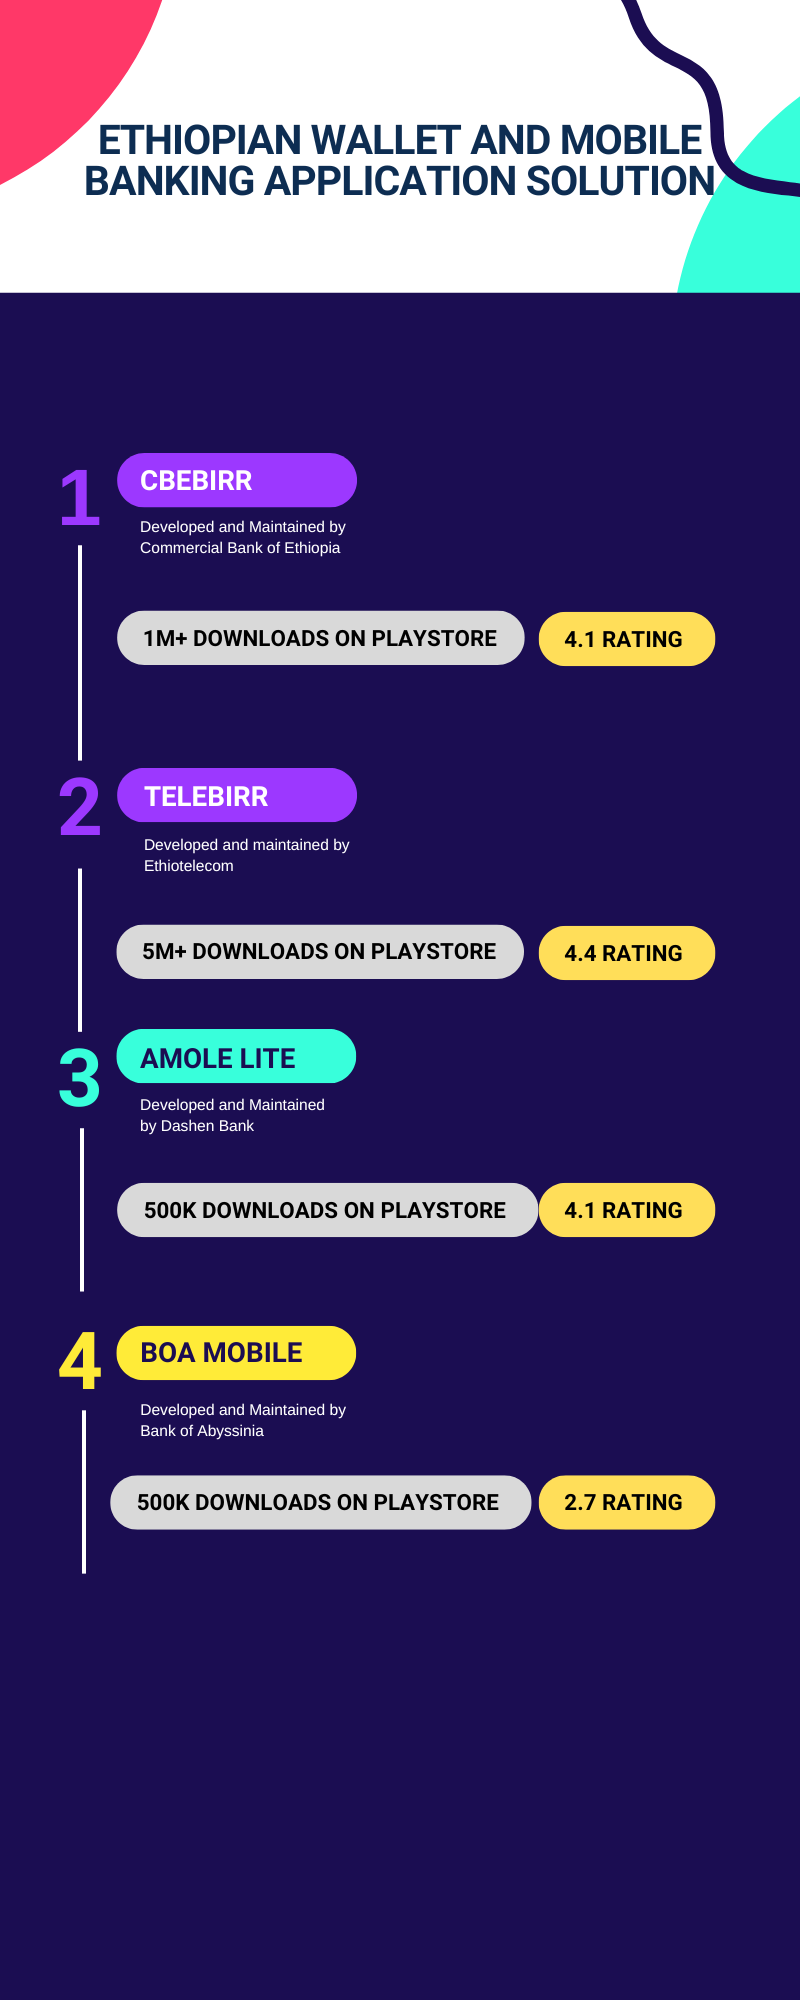
\includegraphics[width=150px]{../images/infographics/apps_basic-statistics.png}
  \caption{Ethiopian Online Banking Solutions}
\end{figure}

\subsection{Comparative Analysis}
\subsubsection{Commercial Bank of Ethiopia CBEBirr}
CBE Birr’s mobile interface demonstrates a modest level of HCI awareness through its use of adaptive keyboards for relevant input fields, effective iconography, and shallow interaction hierarchies, which can reduce cognitive load and task completion time for users. Its relatively polished UI contributes positively to aesthetic–usability effects, making users perceive it as more usable. However, the app significantly lacks in accessibility and customization features, especially critical for elderly and novice users. The absence of a startup language selector and limited language support (only Amharic and English) restricts inclusiveness for Ethiopia’s linguistically diverse population. Additionally, small text, non-scalable typography, and dense layouts present visual and motor challenges, particularly for users with declining vision or limited dexterity. Crowded interfaces and non-prominent help/contact features further hinder error recovery and user confidence. Despite its visual appeal, CBE Birr falls short in accommodating diverse user capabilities, making it less usable for the very demographics this project aims to support.

\begin{figure}[h]
  \centering
  \begin{minipage}[b]{0.3\textwidth}
    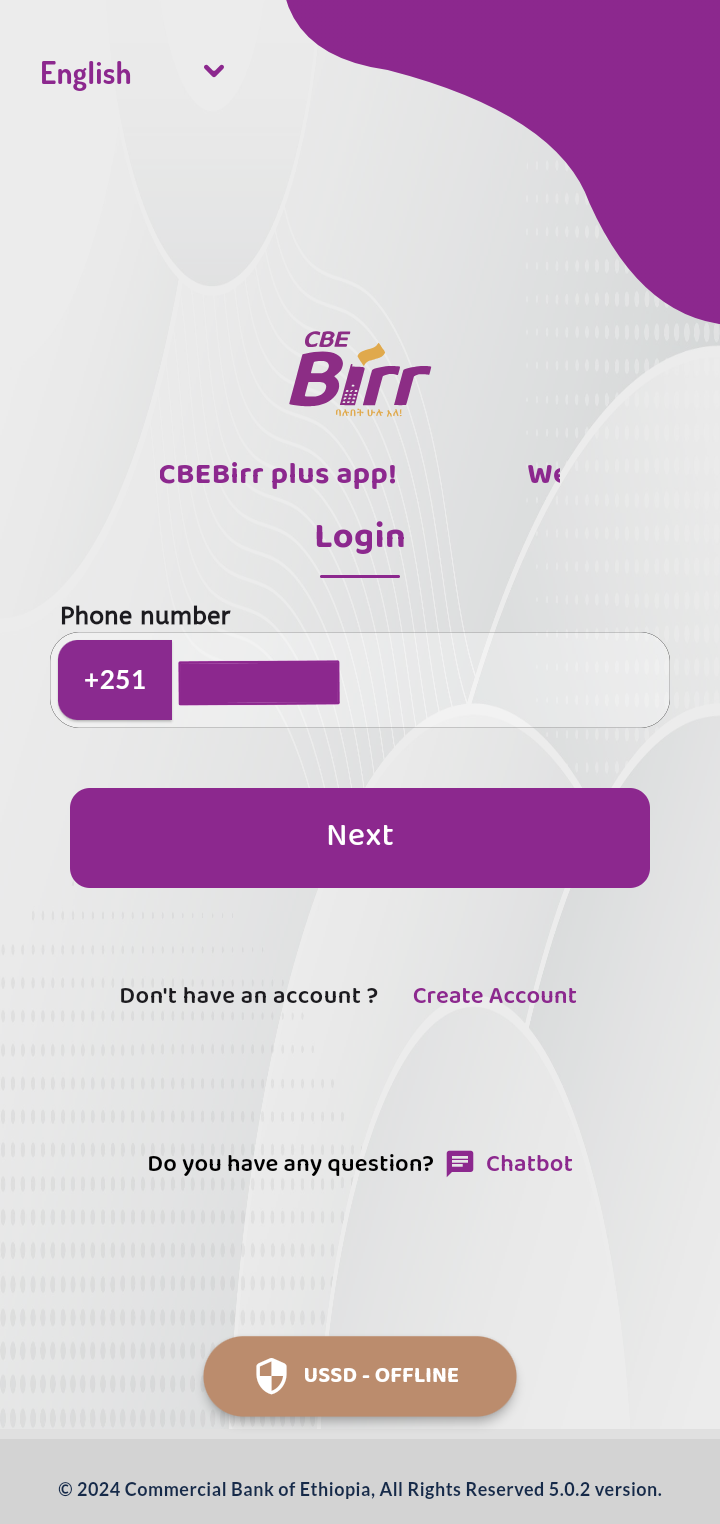
\includegraphics[width=\linewidth]{../images/screenshots/cbebirr/cbebirr_login.png}
    \caption{Login}
  \end{minipage}
  \hfill
  \begin{minipage}[b]{0.3\textwidth}
    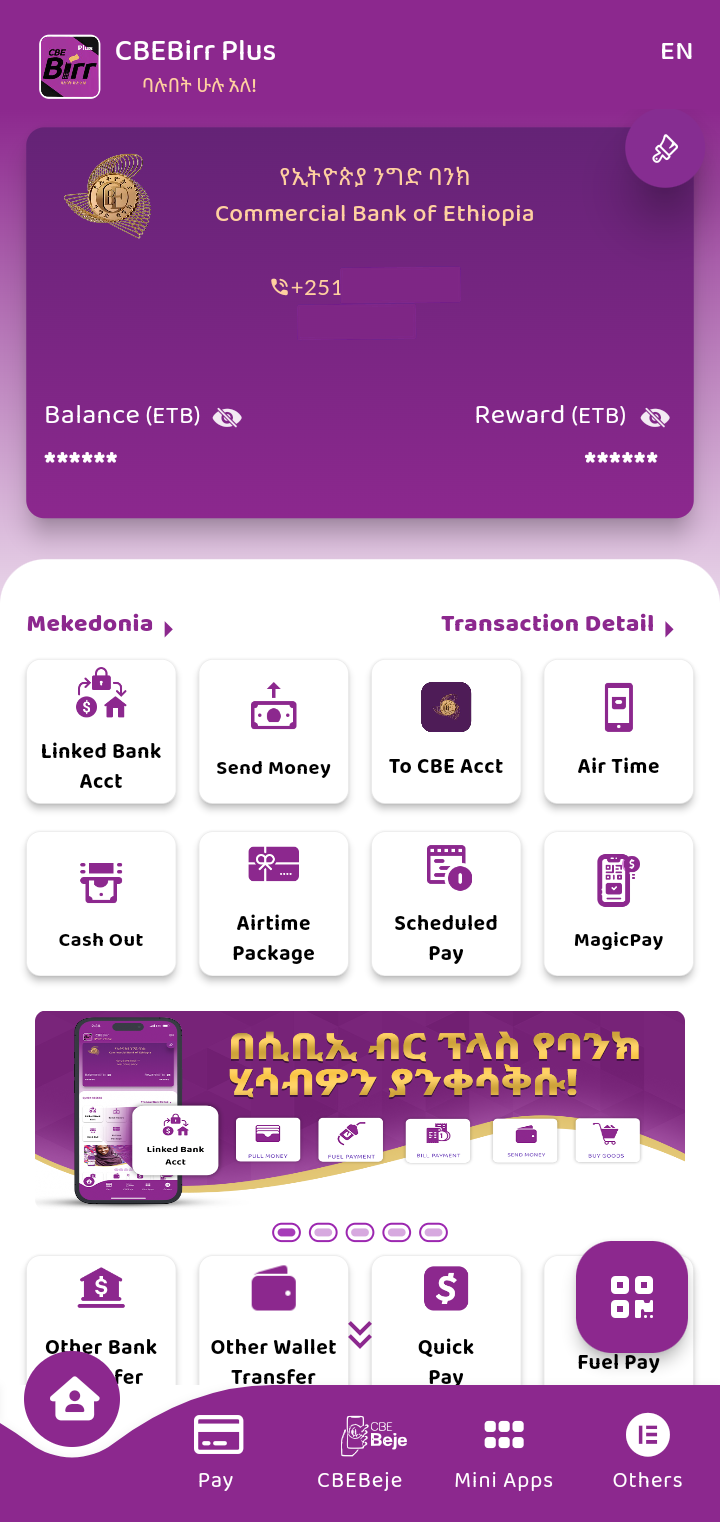
\includegraphics[width=\linewidth]{../images/screenshots/cbebirr/cbebirr_home.png}
    \caption{Home}
  \end{minipage}
  \hfill
  \begin{minipage}[b]{0.3\textwidth}
    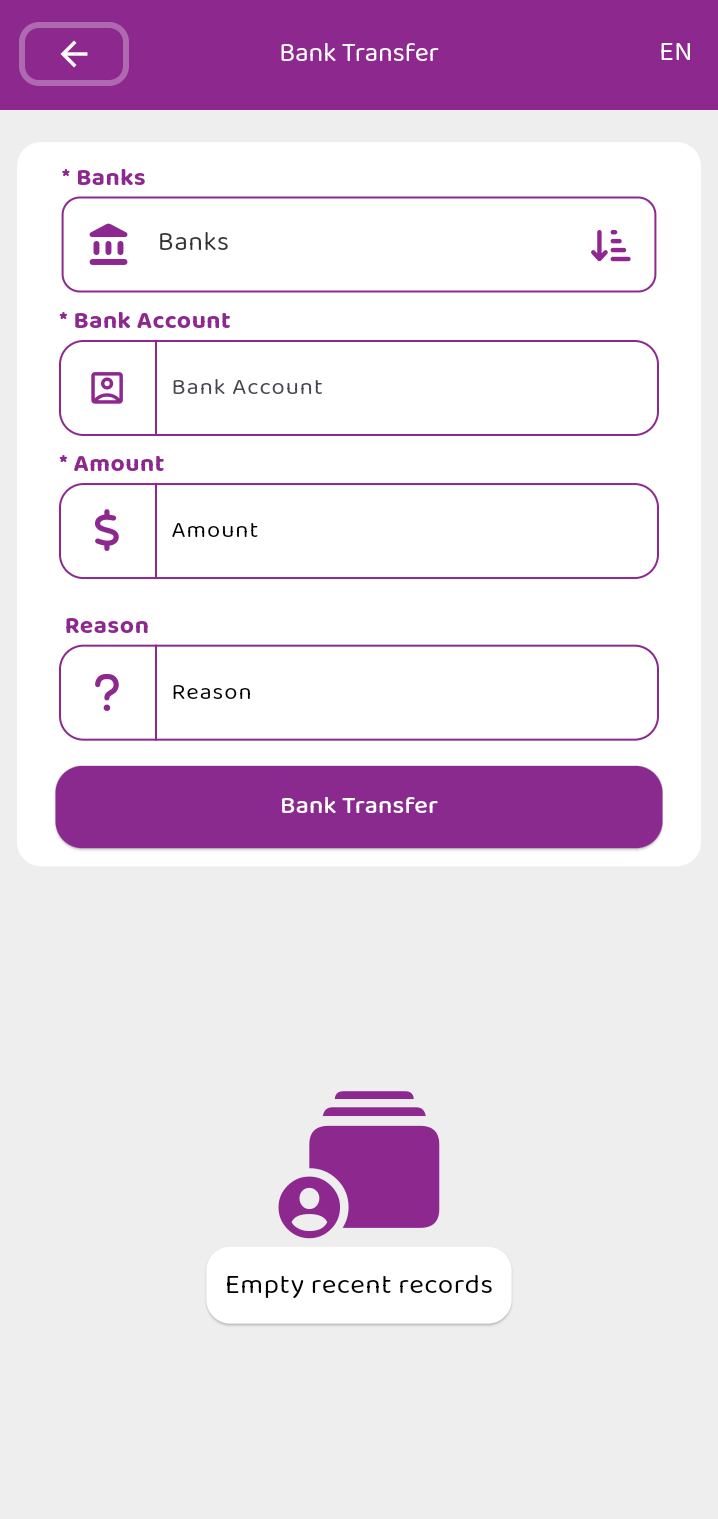
\includegraphics[width=\linewidth]{../images/screenshots/cbebirr/cbebirr_transfers.png}
    \caption{Transfers}
  \end{minipage}
\end{figure}

\subsubsection{Ethiotelecom TeleBirr}
Telebirr offers a few foundational usability strengths, such as adaptive keyboards, reduced interaction depth for key actions, and a broader range of login options and language support, which improve accessibility and task initiation. However, the lack of a startup language selector undermines the utility of its language diversity, especially for first-time users. The interface suffers from visual clutter, with an overloaded home screen that includes rarely used features, increasing cognitive load and reducing task visibility. Small buttons and inconsistent text sizes compound the problem for users with reduced motor control or vision, and the absence of customizable themes or text scaling options further alienates elderly users. Poor icon selection compromises recognition-based navigation, essential for users with low digital literacy. While functional in scope, Telebirr’s interface lacks the simplicity, consistency, and flexibility necessary for inclusive mobile banking experiences.

\begin{figure}[h]
  \centering
  \begin{minipage}[b]{0.3\textwidth}
    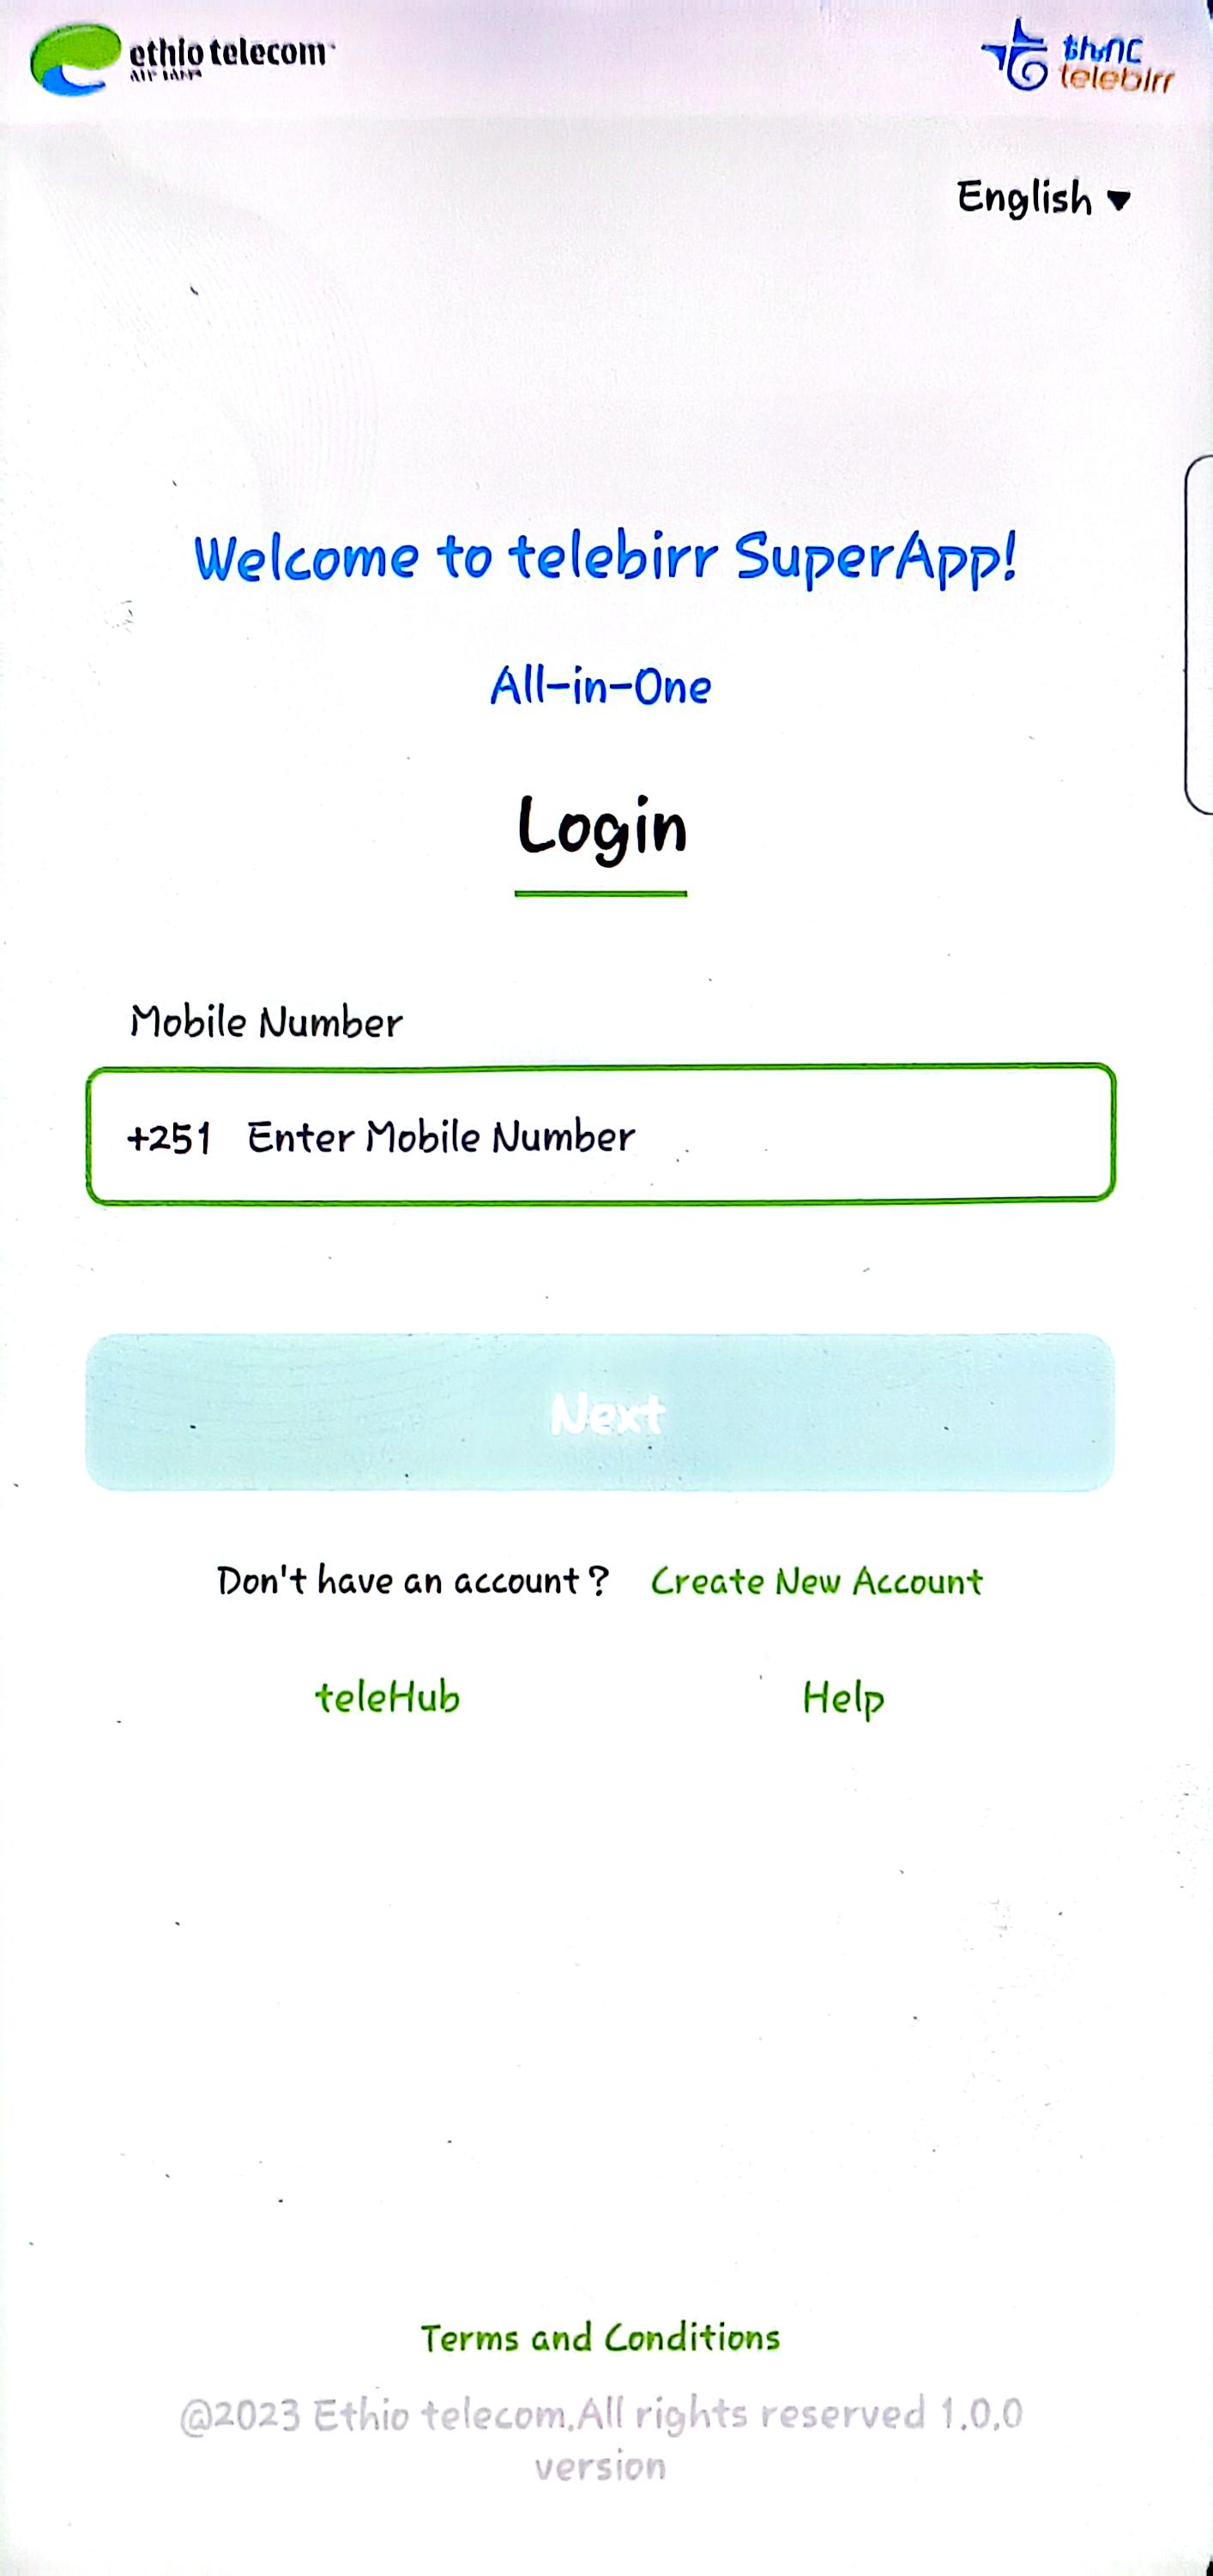
\includegraphics[width=\linewidth]{../images/screenshots/telebirr/telebirr_login.jpg}
    \caption{Login}
  \end{minipage}
  \hfill
  \begin{minipage}[b]{0.3\textwidth}
    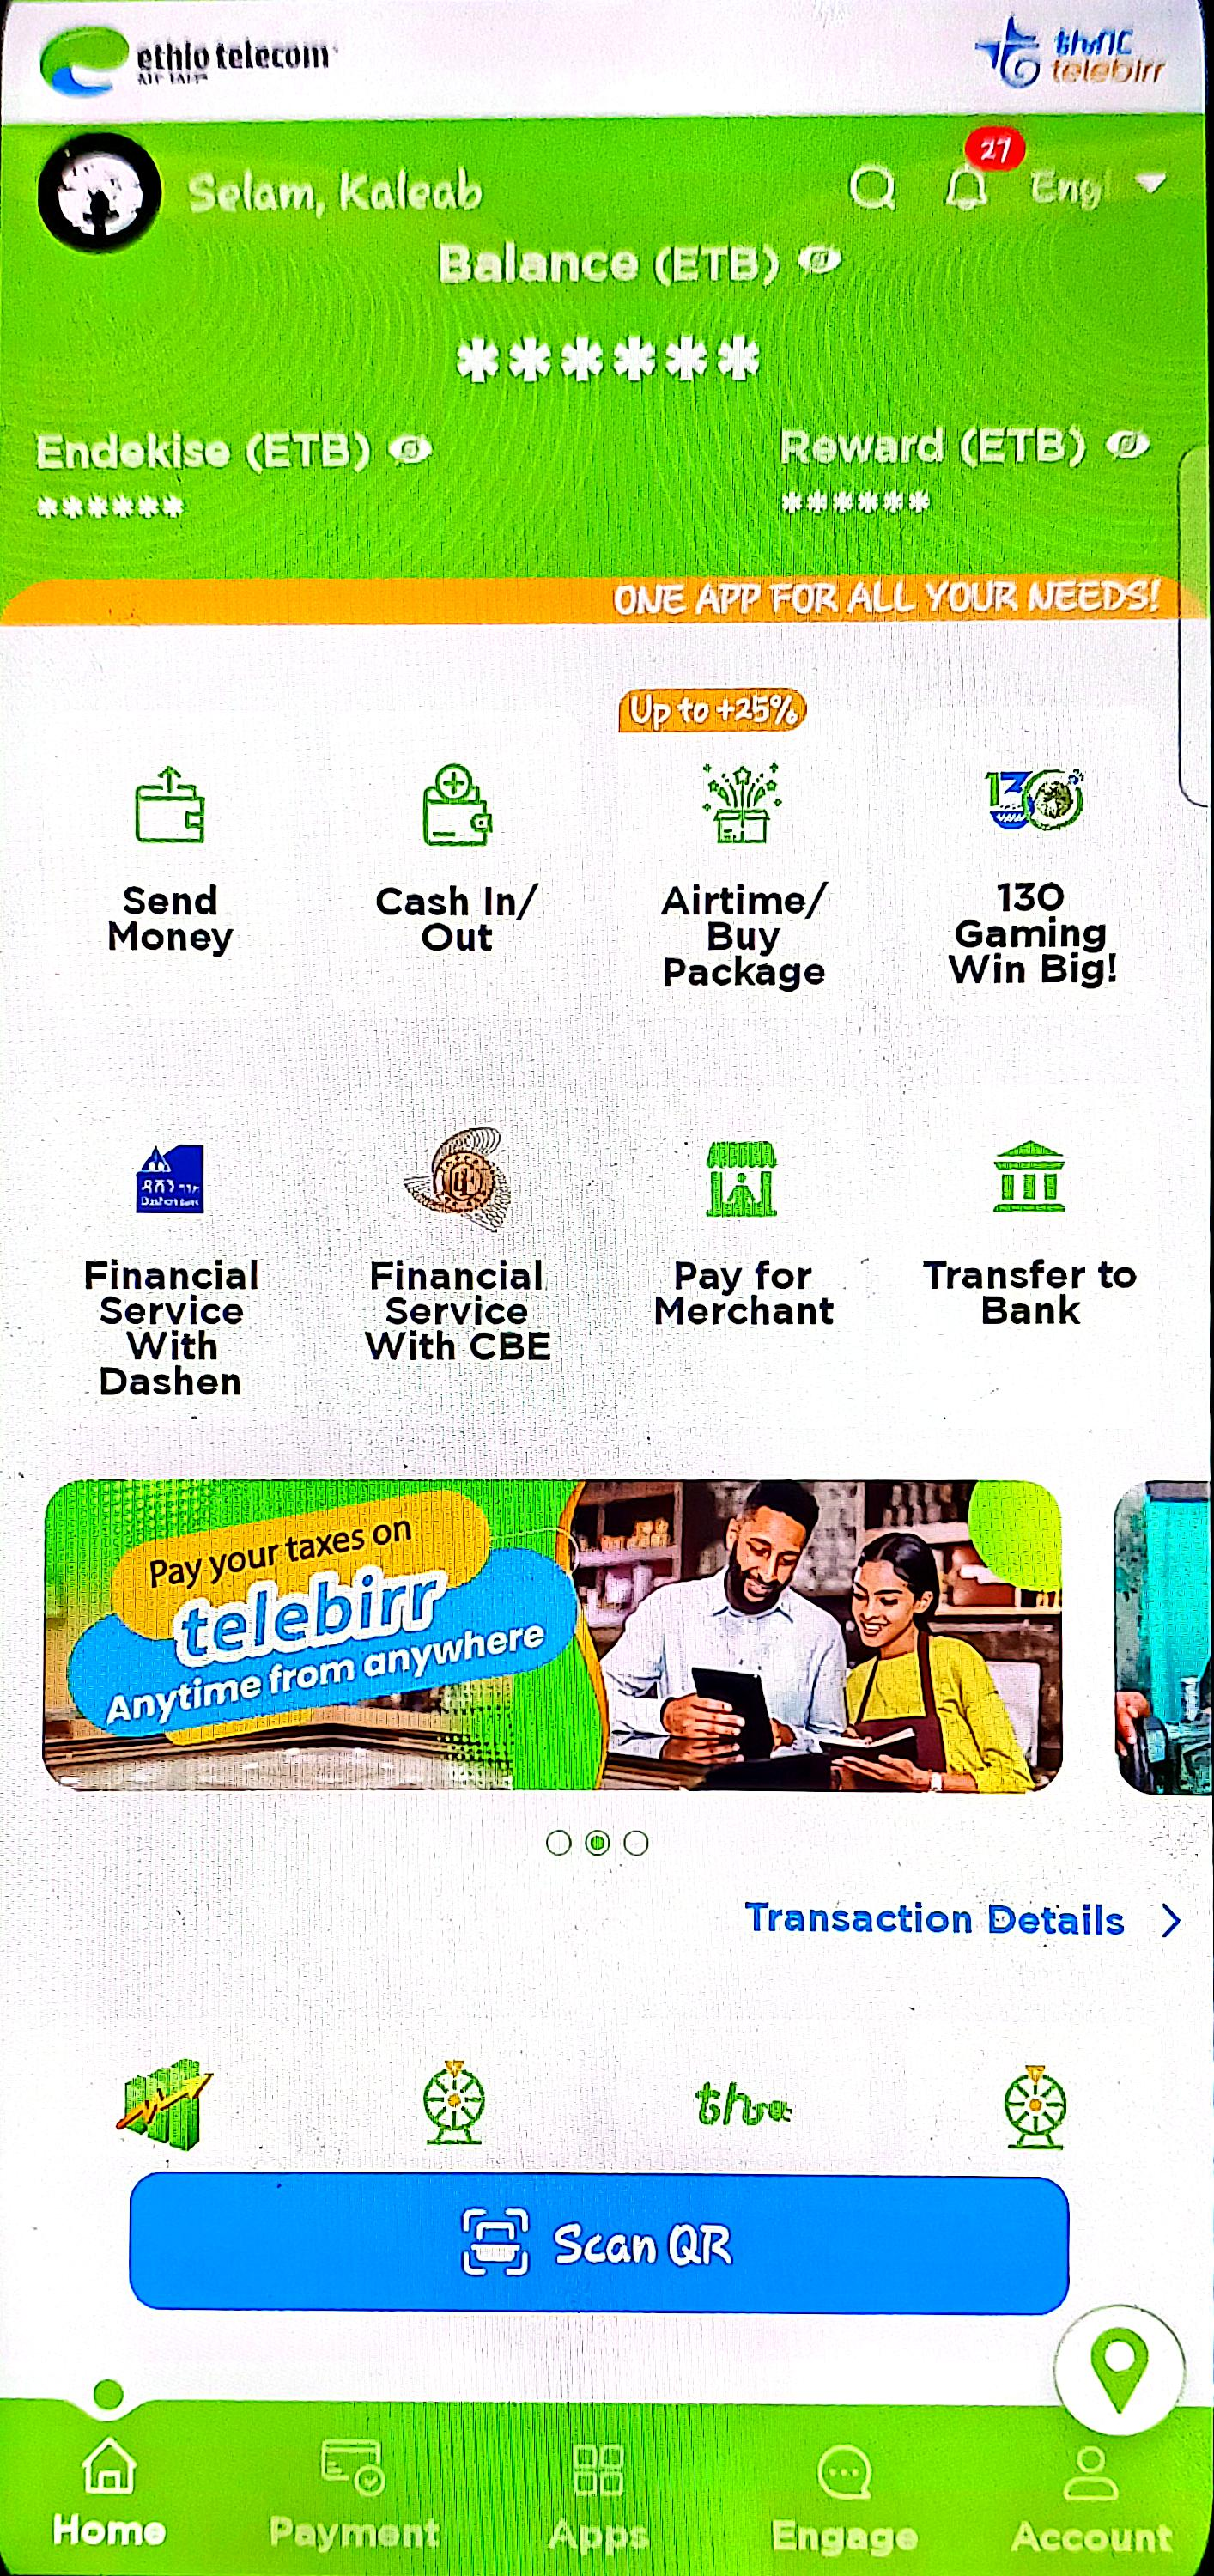
\includegraphics[width=\linewidth]{../images/screenshots/telebirr/telebirr_home.jpg}
    \caption{Home}
  \end{minipage}
  \hfill
  \begin{minipage}[b]{0.3\textwidth}
    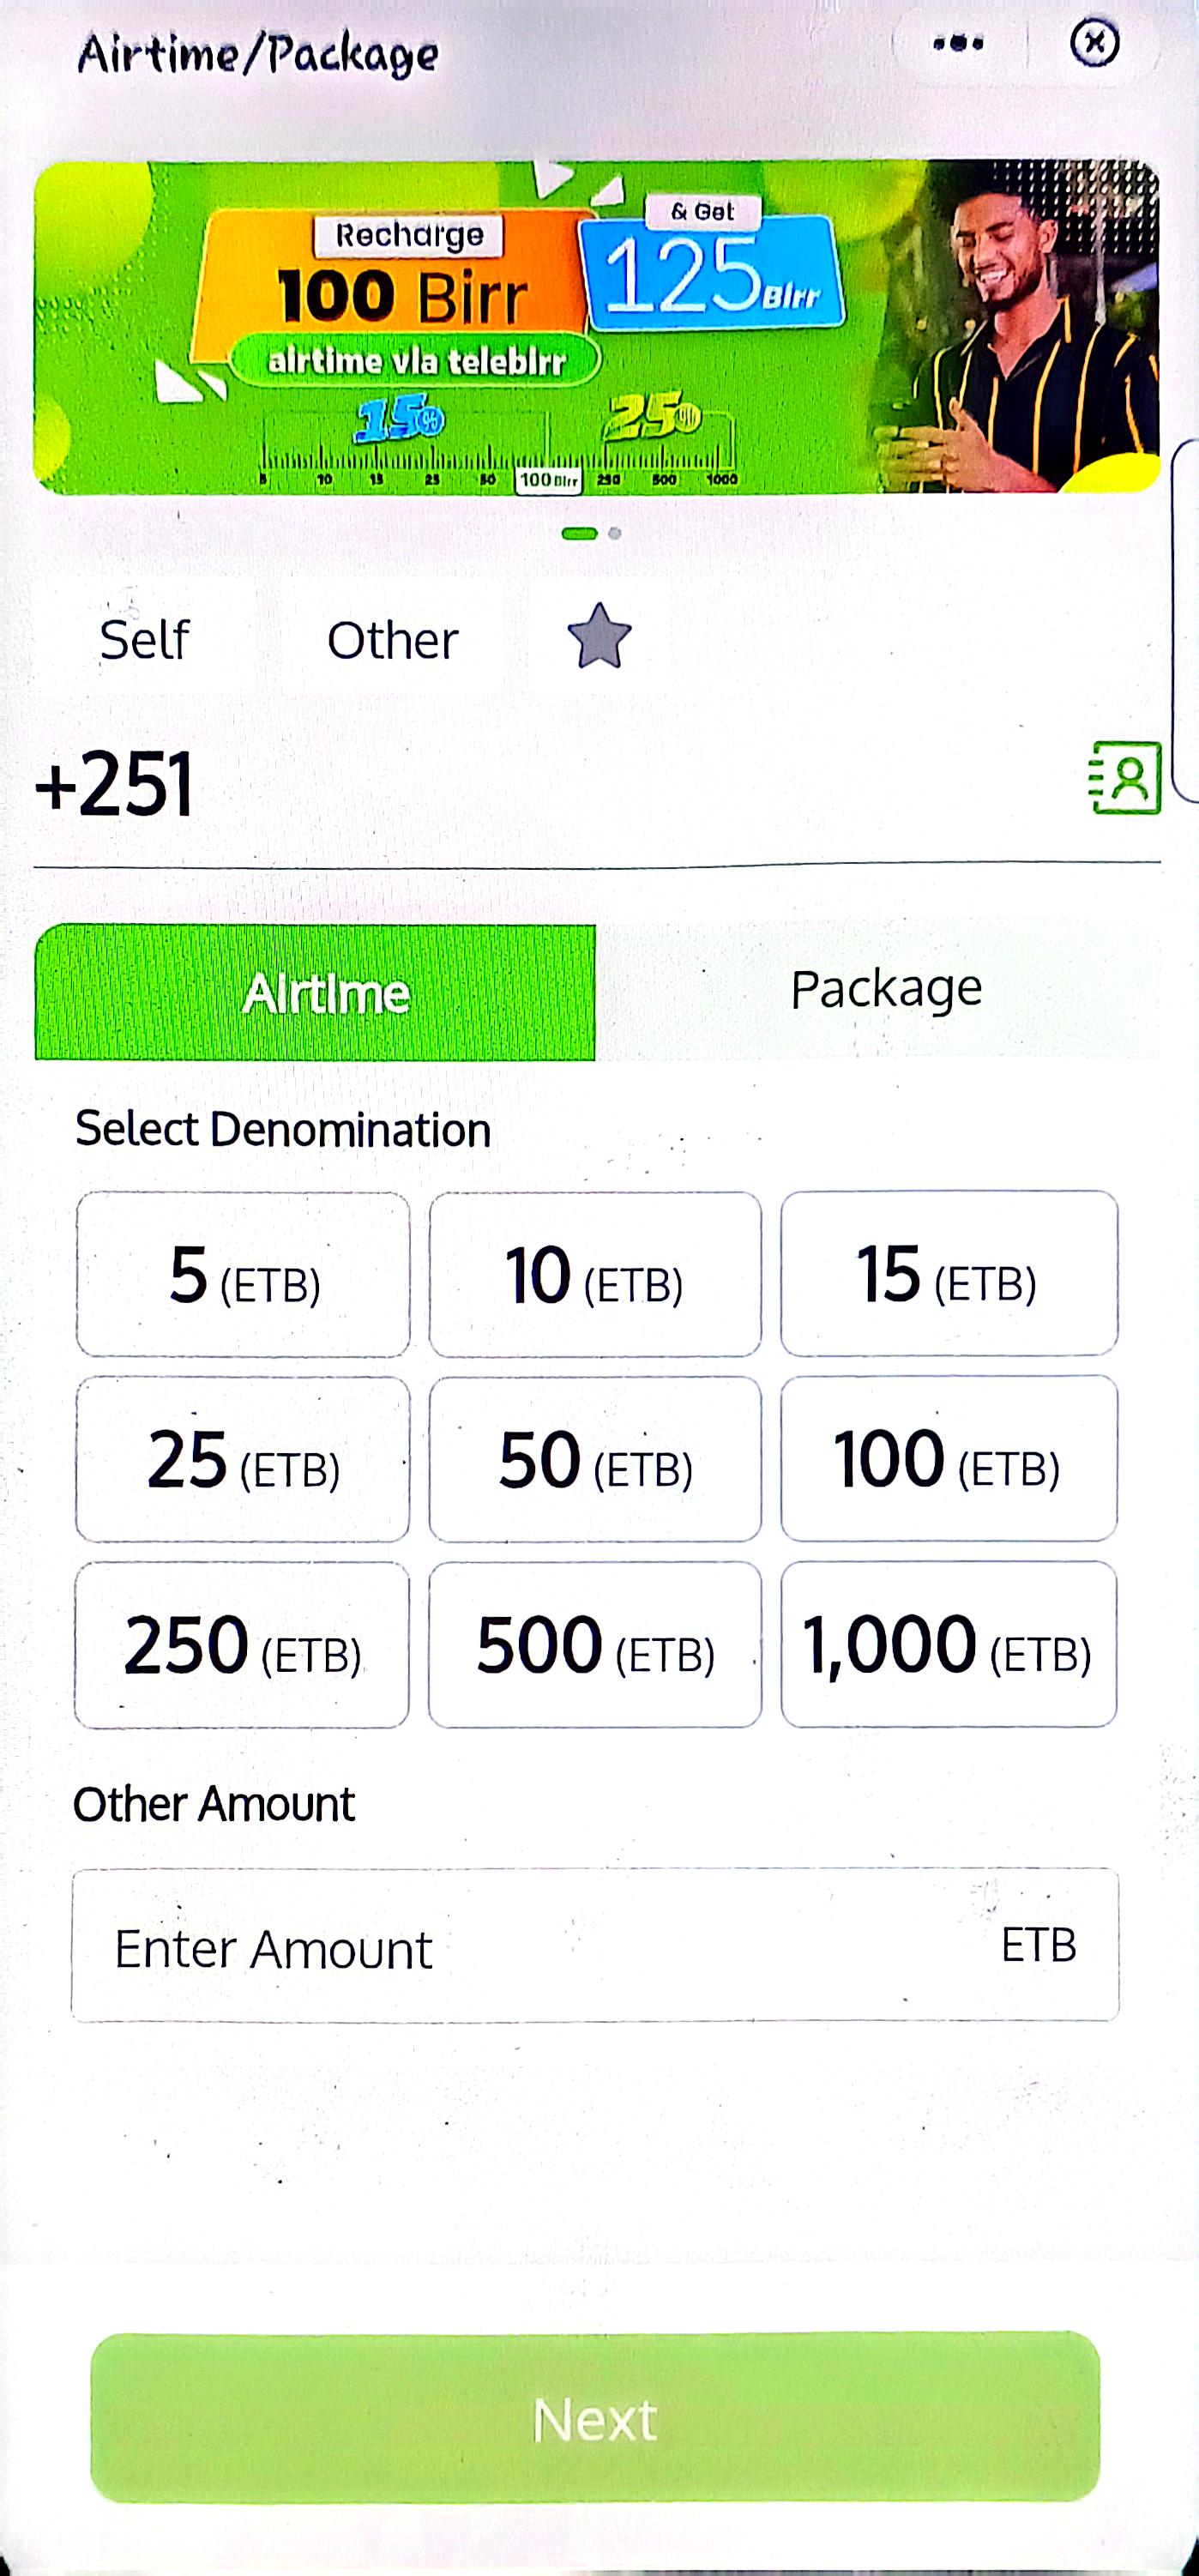
\includegraphics[width=\linewidth]{../images/screenshots/telebirr/telebirr_airtime-topup.jpg}
    \caption{Transfers}
  \end{minipage}
\end{figure}

\subsubsection{Bank of Abyssinia Mobile Banking}
Bank of Abyssinia’s mobile app attempts to support basic usability through larger iconography, wider button spacing, and a relatively clean screen layout, which can help reduce errors for users with motor or cognitive limitations. Its multiple login methods and diversified language options suggest a degree of inclusiveness. However, the benefits are undermined by a lack of startup language selection, forcing users into default choices that may not match their preferences. Critically, frequently used tasks like money transfer are buried under deep interaction paths, making the app inefficient and difficult to learn — a key barrier for novice users. Inconsistent keyboard behavior, along with small, dense text and jargon-heavy labels, compromises readability and discoverability. The inability to adjust text size or theme adds to the inaccessibility. While spatial design is more forgiving, BOA’s mobile app falls short in learnability, error prevention, and adaptability, resulting in a frustrating experience for users who need simplicity and clarity the most.

\begin{figure}[h]
  \centering
  \begin{minipage}[b]{0.3\textwidth}
    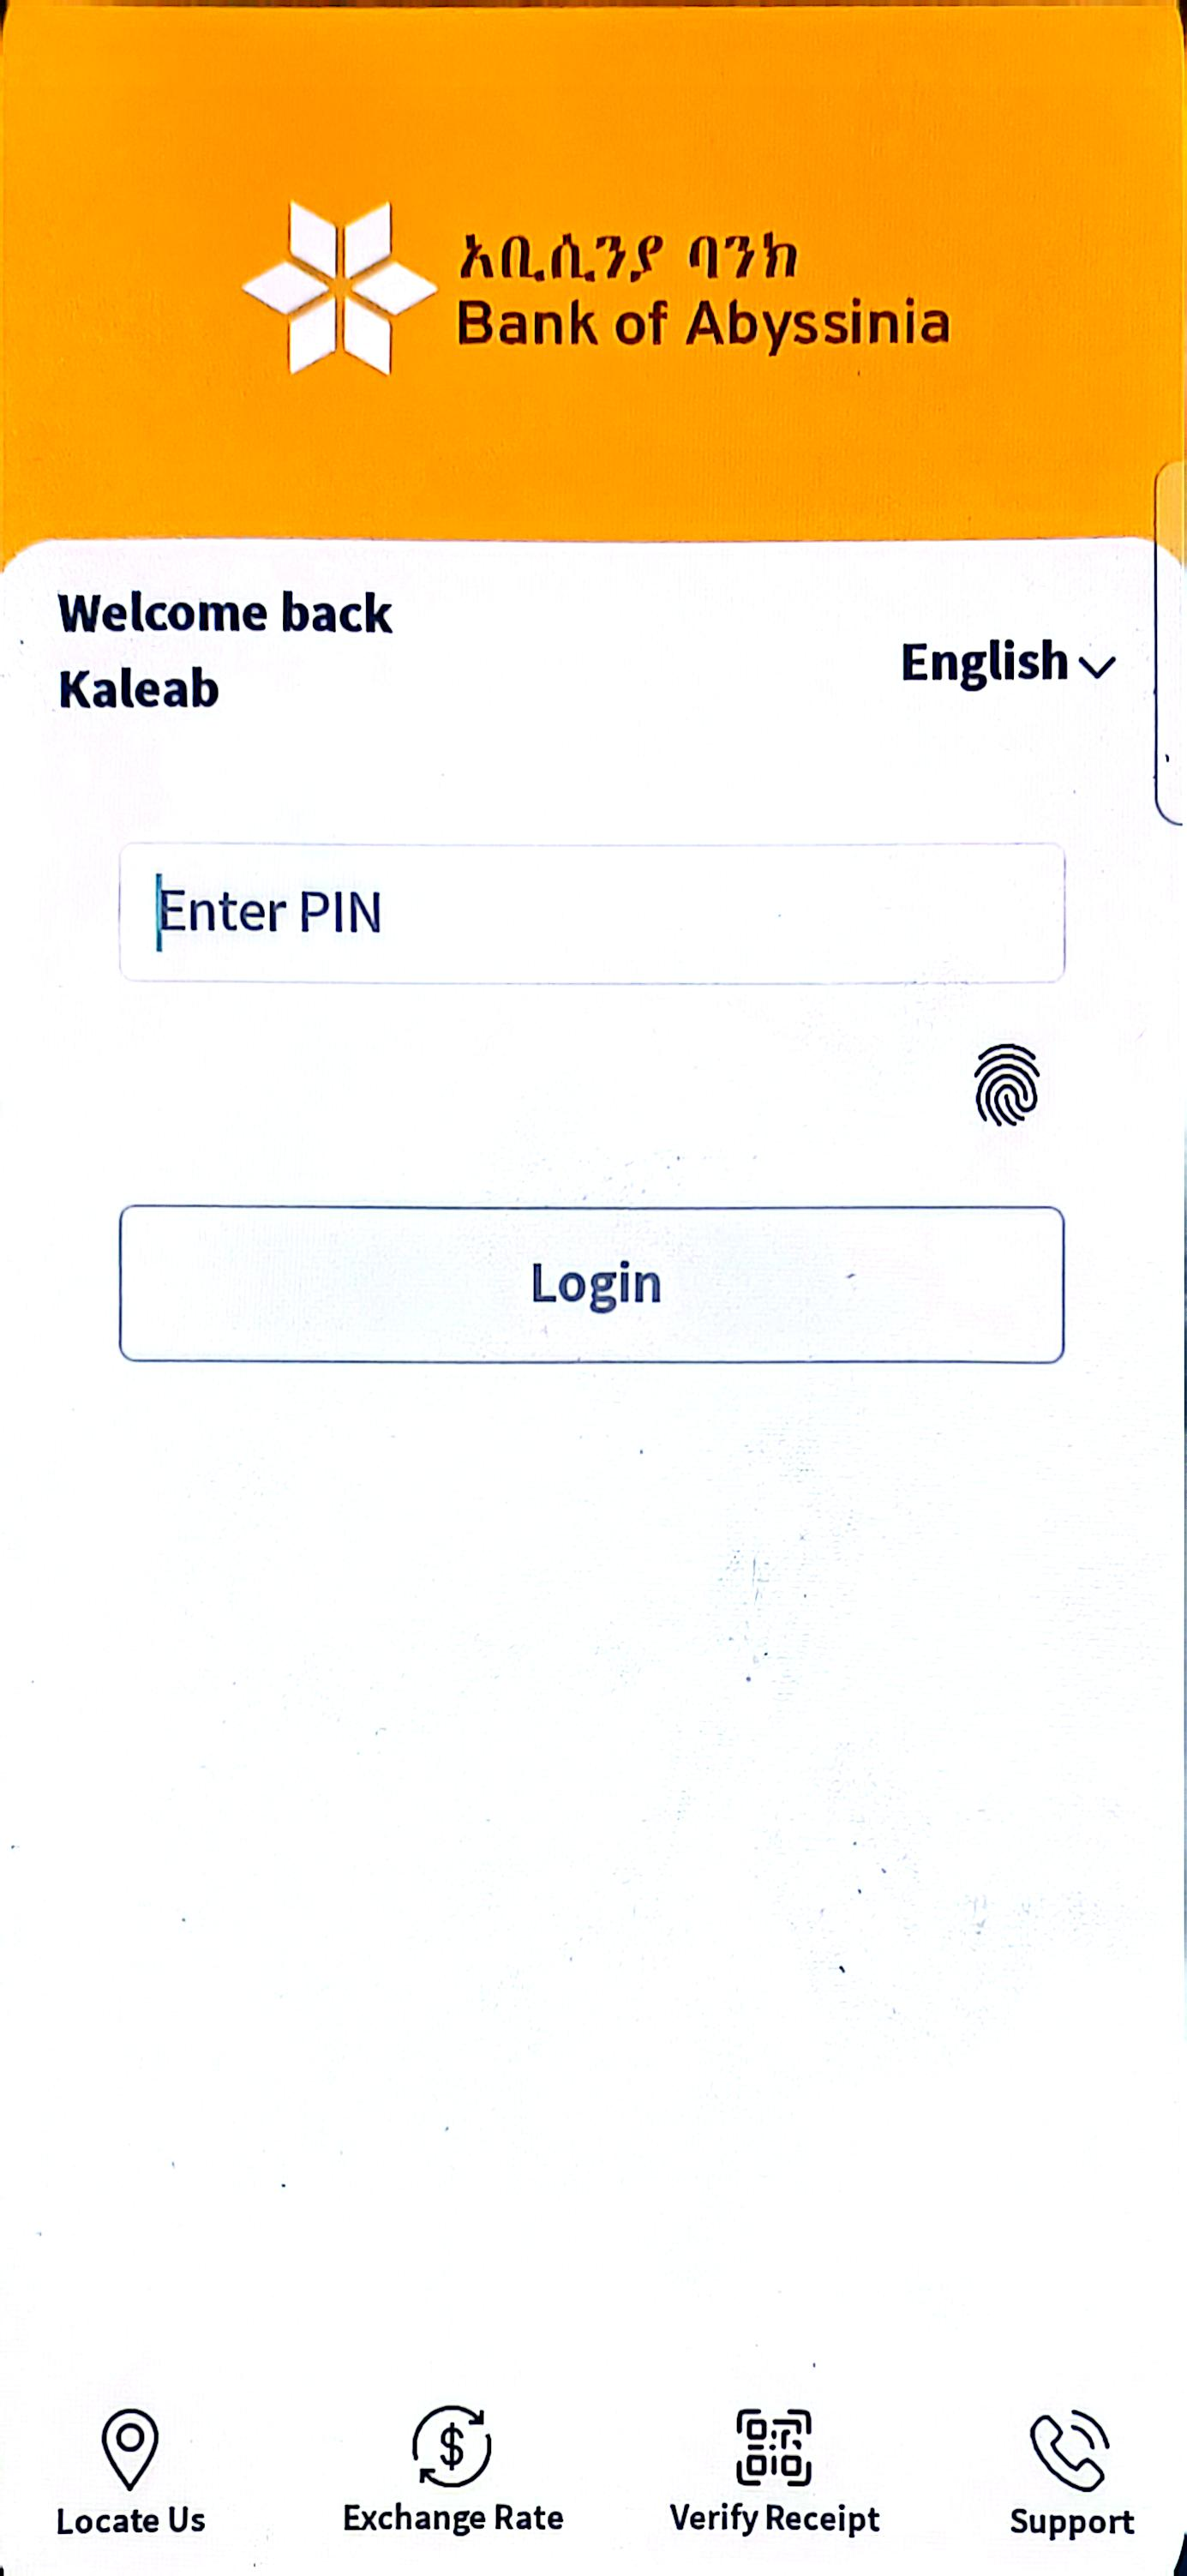
\includegraphics[width=\linewidth]{../images/screenshots/bank-of-abyssinia/boa_sign-in.jpg}
    \caption{Login}
  \end{minipage}
  \hfill
  \begin{minipage}[b]{0.3\textwidth}
    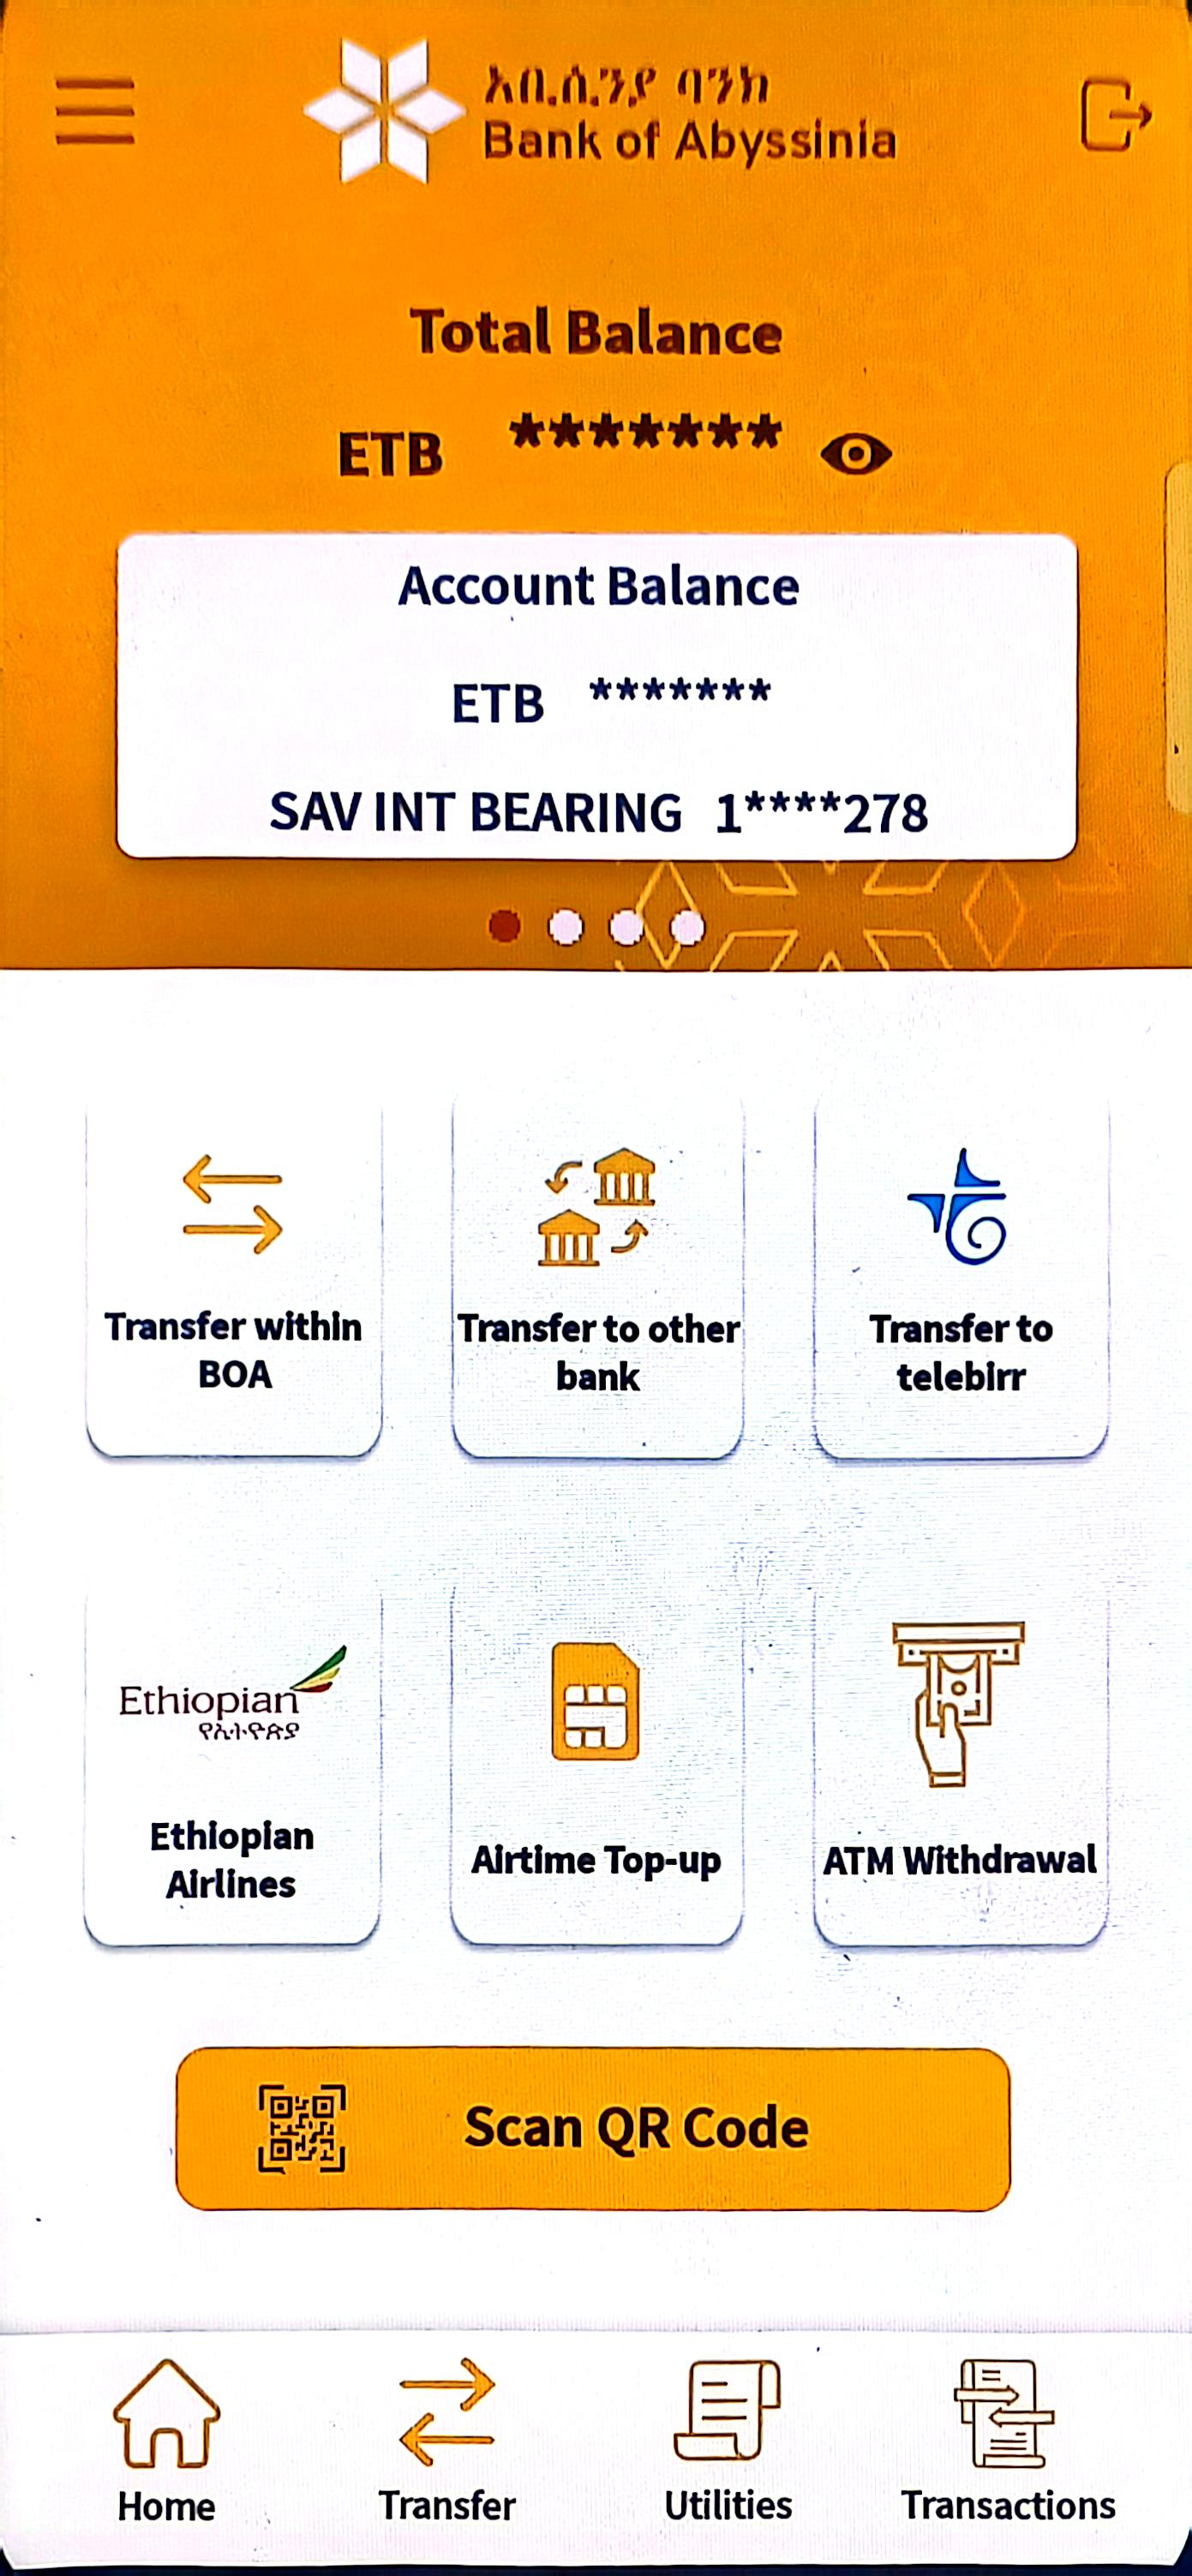
\includegraphics[width=\linewidth]{../images/screenshots/bank-of-abyssinia/boa_home.jpg}
    \caption{Home}
  \end{minipage}
  \hfill
  \begin{minipage}[b]{0.3\textwidth}
    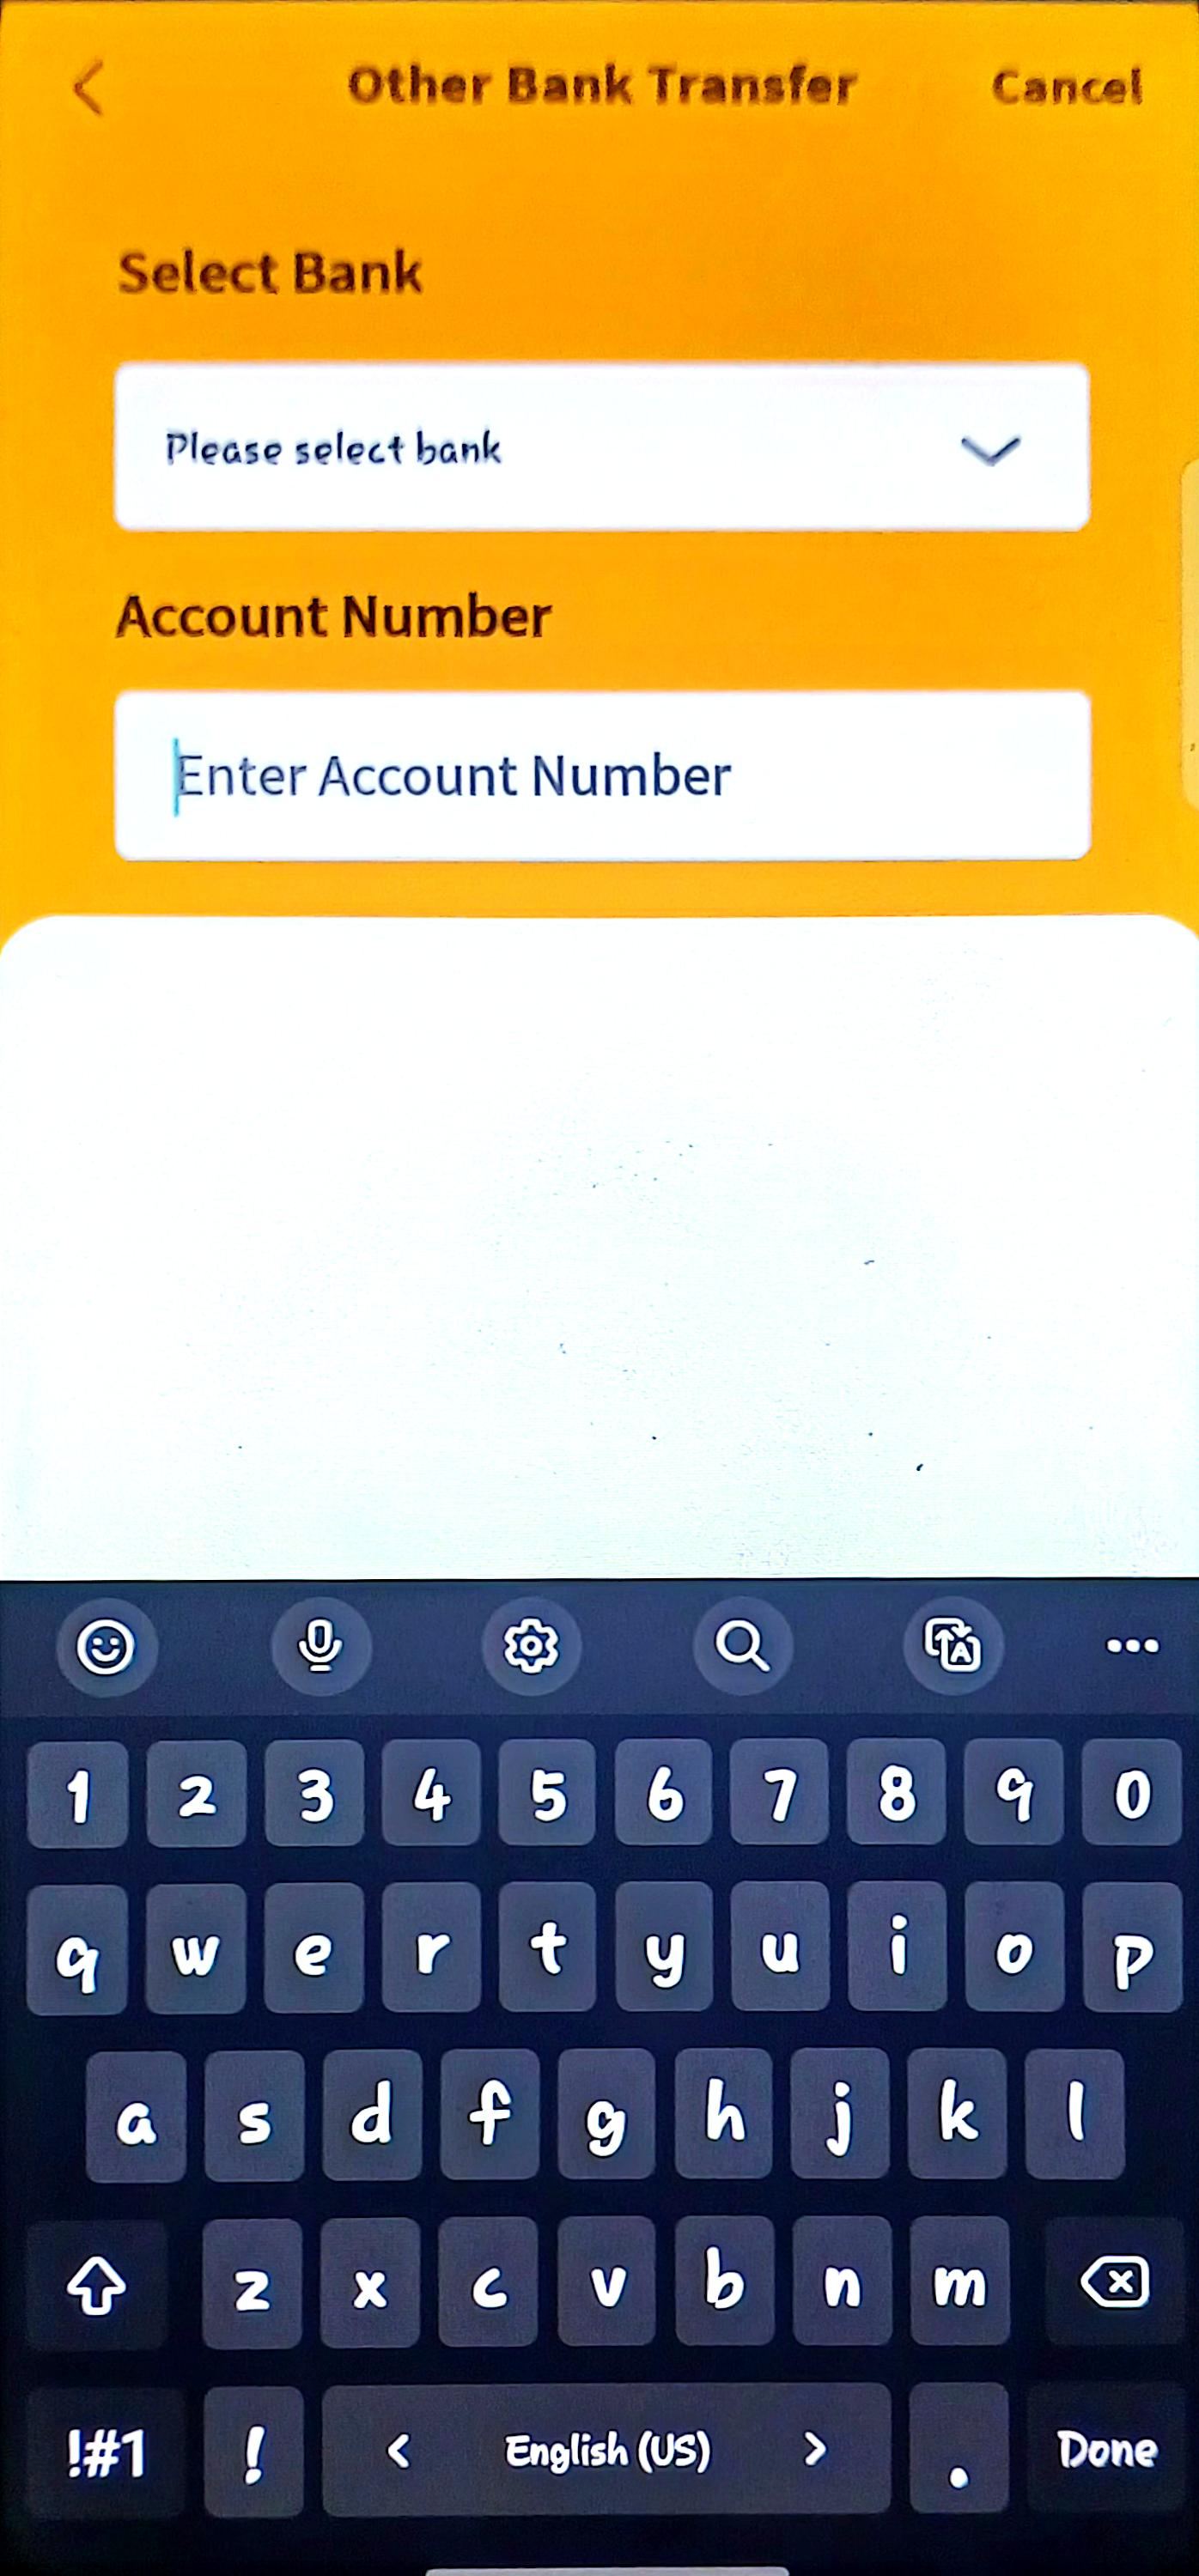
\includegraphics[width=\linewidth]{../images/screenshots/bank-of-abyssinia/boa_transfer.jpg}
    \caption{Transfers}
  \end{minipage}
\end{figure}

\subsubsection{Dashen Bank Amole Lite}
Amole Lite stands out modestly in spatial layout, offering wider button spacing and less visual clutter, which aligns better with the perceptual and motor needs of elderly users. It supports a good number of login options and diverse language support, theoretically enhancing accessibility. However, the lack of an initial language selector and the rigid login process—which demands full credentials every time—introduce significant usability friction. The app’s use of a generic alphabetic keyboard regardless of context increases interaction cost and cognitive load, particularly for users unfamiliar with smartphone conventions. OTP verification for every transaction, while secure, may overwhelm less tech-savvy users. Additionally, the small and unscalable text, absence of theming, and use of ambiguous icons and labels impede readability and navigation. The obscured ‘Contact Us’ option further restricts help-seeking behavior. Though spatially accommodating, Amole Lite fails to deliver on flexibility, simplicity, and user control—critical pillars for a universally usable banking experience.

\begin{figure}[h]
  \centering
  \begin{minipage}[b]{0.3\textwidth}
    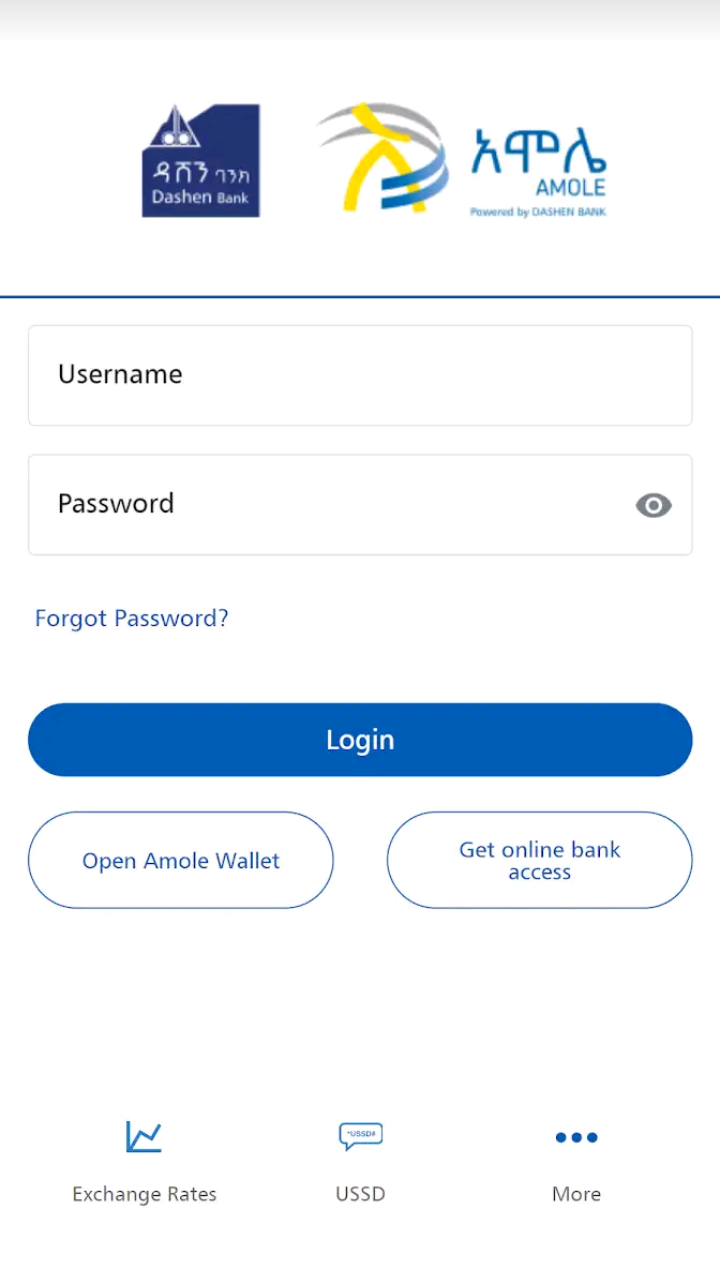
\includegraphics[width=\linewidth]{../images/screenshots/amole-lite/amole_login.png}
    \caption{Login}
  \end{minipage}
  \hfill
  \begin{minipage}[b]{0.3\textwidth}
    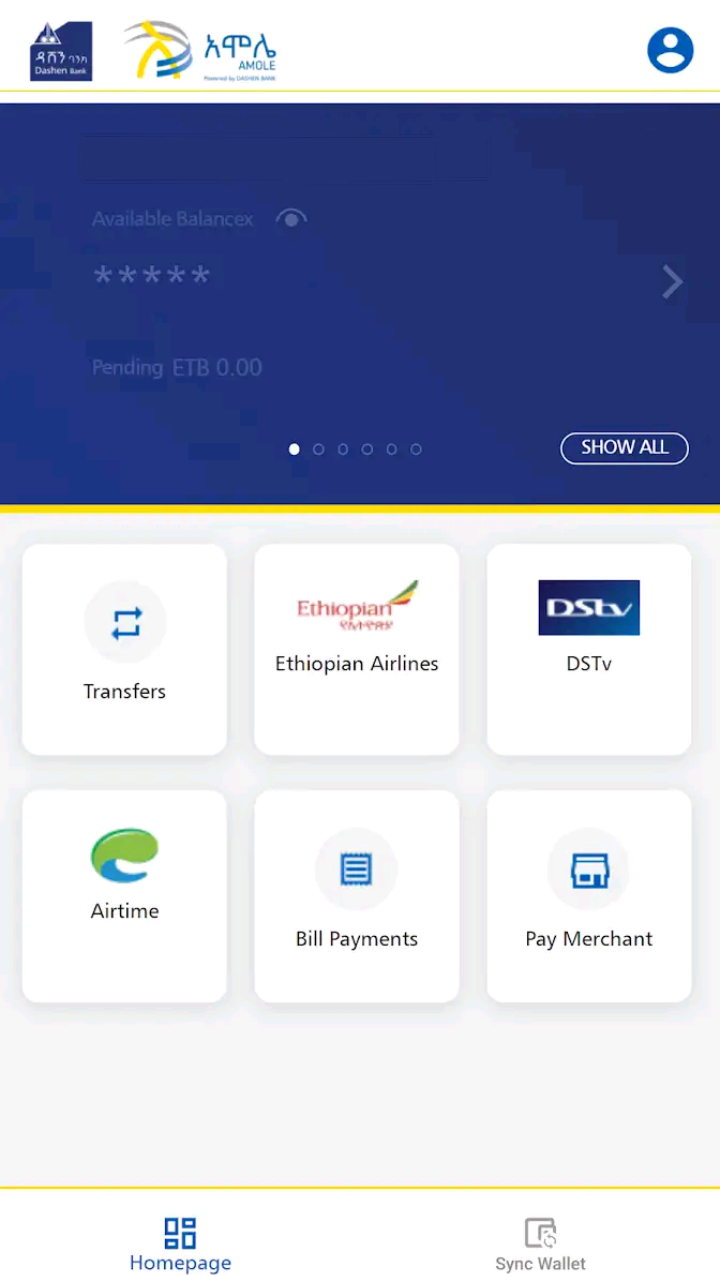
\includegraphics[width=\linewidth]{../images/screenshots/amole-lite/amole_home.png}
    \caption{Home}
  \end{minipage}
  \hfill
  \begin{minipage}[b]{0.3\textwidth}
    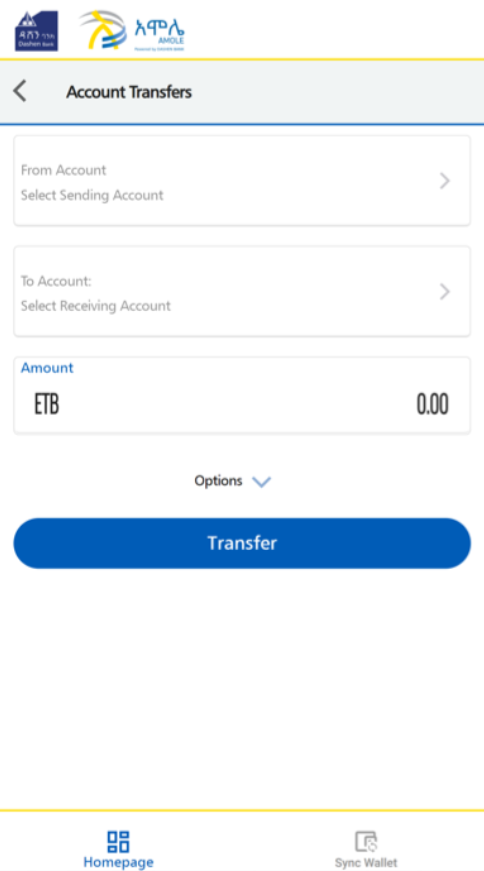
\includegraphics[width=\linewidth]{../images/screenshots/amole-lite/amole_transfers.png}
    \caption{Transfers}
  \end{minipage}
\end{figure}

\subsection{A Good and "Loose" Frame of Reference - Bank of America}
Bank of America's mobile banking application serves as a loose yet insightful frame of reference for what inclusive and user-friendly mobile financial services could look like when grounded in core HCI principles such as perceptibility, low memory burden, and error recovery. The application embraces a user-centered design approach, explicitly tailoring the experience for elderly and novice users—two demographics that often face cognitive and sensory barriers in mobile interfaces. For example, the inclusion of an *Easy Mode* follows the principle of progressive disclosure, reducing cognitive load by surfacing only essential features and using bold typography and large buttons to align with Fitts’s Law and the needs of users with visual or motor impairments. Its voice-controlled assistant, Erica, supports natural language input, lowering interaction friction for users with limited dexterity or digital literacy, reflecting multimodal interaction principles. The app also supports adaptive interfaces, such as dynamic font scaling and high-contrast UI themes, ensuring perceptibility across varying physical and environmental conditions—a direct application of universal design.

Moreover, the system offloads memory demand through biometric authentication and customizable home screens, effectively reducing recognition over recall, and providing shortcuts for routine tasks—critical for elderly users with decreased working memory. Real-time fraud alerts and instant card freezing mechanisms integrate feedback and control visibility, helping users feel secure and in charge. Tutorials and demo modes facilitate learnability and error tolerance, which are essential for building confidence among tech novices. Collectively, these features illustrate a design that doesn’t just accommodate impairments but actively enhances usability by empowering users, making it a valuable referential benchmark as we critically analyze and rethink the status quo of Ethiopian mobile banking solutions.

\subsection{Comparison With Our Frame of Reference}

When comparing generalized Ethiopian mobile banking apps to Bank of America’s mobile banking application, several key differences emerge in terms of usability, accessibility, and inclusivity, particularly for elderly and novice users:

\begin{itemize}[label=--]
  \item \textbf{Information Architecture}:
        Ethiopian apps like CBE Birr and Telebirr tend to have cluttered interfaces with deep interaction nesting, which makes it difficult for users to quickly complete tasks. In contrast, Bank of America offers an \textbf{Easy Mode}, which simplifies the interface and prioritizes essential functions, reducing cognitive load.

  \item \textbf{Multimodal Interaction}:
        Ethiopian apps often lack \textbf{voice control} and adaptive features for users with motor impairments or those unfamiliar with touch-based interfaces. Bank of America, however, provides \textbf{voice-controlled banking} via Erica, enabling users to perform tasks using natural language commands, which greatly benefits users with limited dexterity.

  \item \textbf{Customization}:
        Ethiopian apps do not support \textbf{text size adjustment} or \textbf{high-contrast modes}, limiting accessibility for visually impaired users. Bank of America offers adjustable text sizes and a \textbf{high-contrast UI}, allowing users to customize the app according to their visual needs.

  \item \textbf{Authentication and Security}:
        Ethiopian apps rely on traditional \textbf{username/password} authentication, which can be cumbersome for elderly users. Bank of America uses \textbf{biometric login} (fingerprint and face ID), simplifying access while improving security. The app also offers \textbf{real-time fraud alerts} and the ability to freeze debit cards instantly.

  \item \textbf{Customer Support and Learnability}:
        Access to customer support in Ethiopian apps is often buried in complex menus. Bank of America, on the other hand, provides \textbf{one-tap customer service} and offers \textbf{tutorials and demo modes}, allowing users to practice in a safe environment and reducing the learning curve.
\end{itemize}

\section{Current Users' Journey}
This user journey map outlines the key cognitive, emotional, and interactional challenges faced by elderly or novice users during the onboarding and adoption phases of a mobile banking app. The journey is broken into three phases: discovery and registration, learning core features, and advanced usage. In the first phase, users often experience discoverability issues and cognitive overload, with the fear of scams and resistance to technology making the process stressful. During the learning phase, mental model mismatches and small text sizes complicate navigation, leading to confusion. As users advance to more independent usage, a lack of reminders and frequent UI changes create discomfort, affecting confidence and continued engagement.

The emotional journey reflects a mix of frustration and relief, with anxiety about security and confusion about navigation being common pain points. Positive emotional peaks occur when users successfully complete tasks and feel a sense of accomplishment. To improve this experience, key design fixes include clearer security signals, adjustable text sizes, more intuitive navigation, and improved customer support access. Additionally, integrating adaptive onboarding and augmented assistance can help guide users through the learning process, while data-driven insights can highlight areas for improvement.

Overall, the analysis reveals the importance of designing mobile banking apps with accessibility and emotional support in mind. Implementing features such as a "Senior Mode," simplified interfaces, and a hybrid support system combining AI and human interaction can significantly enhance the user experience, especially for elderly and novice users.

\begin{figure}[h]
  \centering
  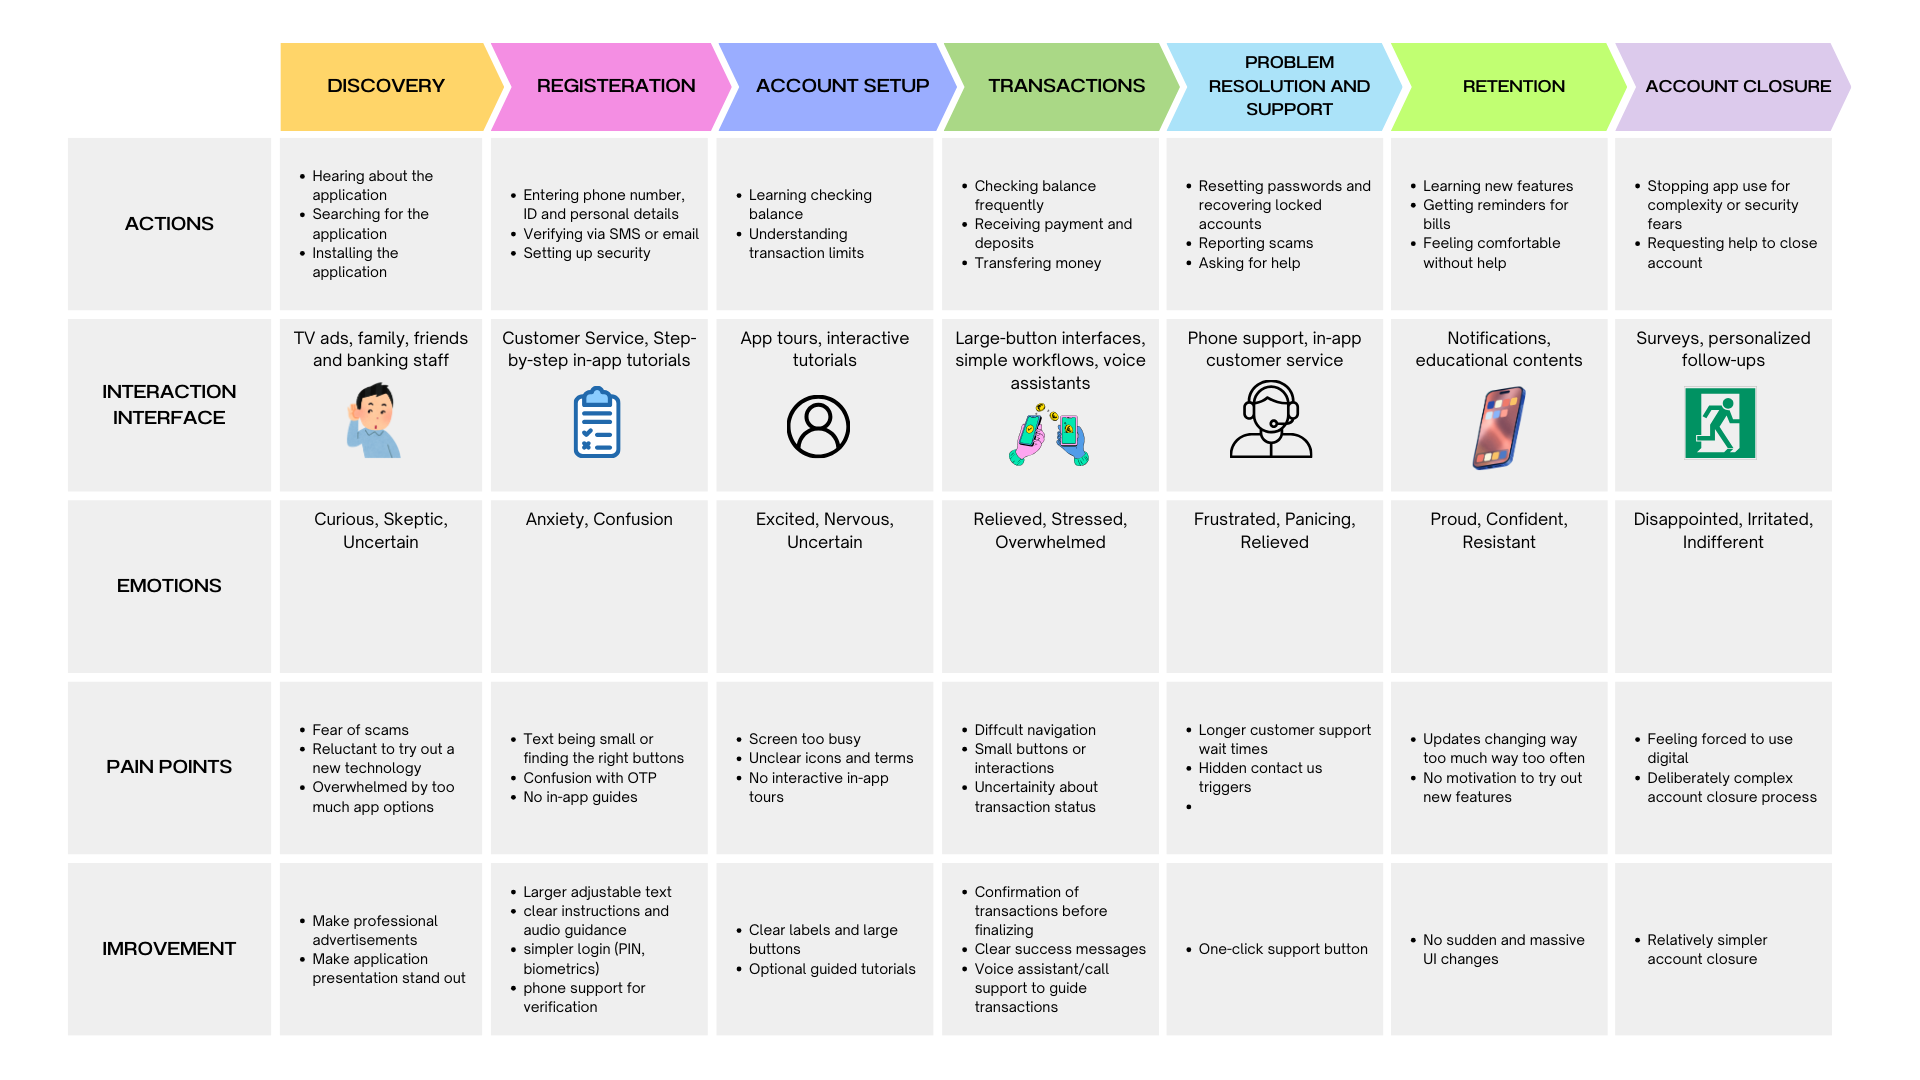
\includegraphics[width=\linewidth]{../images/infographics/user_journey.png}
  \caption{User Journey for an Elderly User}
\end{figure}

\section{Summary: Identified Pain Points and Their Solutions}
\begin{itemize}
  \item \textbf{Pain Point 1: Fear of Scams and Low Trust in Security}
        \begin{itemize}
          \item \textbf{Solution:}
                \begin{itemize}
                  \item Dynamic trust signals, such as "Encrypted session" badges to reinforce security.
                  \item In-app scam education through short videos and interactive quizzes.
                \end{itemize}
        \end{itemize}

  \item \textbf{Pain Point 2: Small Text and Poor Input Controls}
        \begin{itemize}
          \item \textbf{Possible Solution:}
                \begin{itemize}
                  \item Adjustable UI for font scaling (up to 200\%) and larger touch targets (48x48px).
                  \item Voice-guided input for tasks, such as saying "Send \$100 to John" instead of typing.
                \end{itemize}
        \end{itemize}

  \item \textbf{Pain Point 3: Unclear Navigation and Confusing CTAs}
        \begin{itemize}
          \item \textbf{Possible Solution:}
                \begin{itemize}
                  \item High-priority buttons (e.g., "Help") placed at the bottom of the screen.
                  \item Contextual tooltips and guided tours to make navigation clearer and reduce confusion.
                \end{itemize}
        \end{itemize}

  \item \textbf{Pain Point 4: Slow or Difficult Customer Support}
        \begin{itemize}
          \item \textbf{Possible Solution:}
                \begin{itemize}
                  \item One-tap call support or a dedicated support button (e.g., Samsung's Bixby key remapping).
                  \item AI-powered chatbot triage to help users describe issues quickly and connect to an agent.
                \end{itemize}
        \end{itemize}


  \item \textbf{Pain Point 5: Language Support Issues}
        \begin{itemize}
          \item \textbf{Solution:}
                \begin{itemize}
                  \item Provide multi-language support to cater to users from different linguistic backgrounds.
                  \item Offer language preferences during the registration process and integrate auto-language detection where feasible.
                \end{itemize}
        \end{itemize}


  \item \textbf{Pain Point 6: Lack of Personalization and Accessibility Options}
        \begin{itemize}
          \item \textbf{Possible Solution:}
                \begin{itemize}
                  \item Customizable home screen with options to pin frequently used features.
                  \item Adjustable text size and high-contrast color schemes for improved readability.
                \end{itemize}
        \end{itemize}

  \item \textbf{Pain Point 7: Unclear or No Graphical Cues and Icons}
        \begin{itemize}
          \item \textbf{Solution:}
                \begin{itemize}
                  \item Use clear, familiar, and consistent icons across the app for common actions (e.g., home, settings, transactions).
                  \item Provide visual cues such as tooltips or highlighted icons to guide users through different sections.
                \end{itemize}
        \end{itemize}

  \item \textbf{Pain Point 8: Lack of Clear Onboarding and Tutorials}
        \begin{itemize}
          \item \textbf{Possible Solution:}
                \begin{itemize}
                  \item Adaptive onboarding with branching tutorials based on user competence.
                  \item Interactive walkthroughs and demo modes for first-time users, allowing them to practice without real accounts.
                \end{itemize}
        \end{itemize}

\end{itemize}

\newpage
\chapter*{Chapter Two: Usability of Mobile Banking Applications: Literature Review}
\addcontentsline{toc}{chapter}{Usability of Mobile Banking Applications: Literature Review}
\setcounter{chapter}{2}
\setcounter{section}{0}
\section{Introduction}
The purpose of this systematic literature review (SLR) is to gain a comprehensive understanding of usability issues related to elderly and novice users in the context of mobile banking applications. As mobile banking services continue to grow in importance, it is crucial to ensure that these services are accessible and usable for all user groups, particularly those who may face challenges due to their limited experience with technology or cognitive and physical limitations. Elderly and novice users are often overlooked in usability studies, yet they represent significant segments of mobile banking users who struggle with complex interfaces, security concerns, and lack of support.

\begin{itemize}
  \item The first paper focuses on \textbf{general usability} in mobile banking applications, providing insights into common challenges faced by users, and how these affect user satisfaction and retention.
  \item The second paper examines \textbf{usability issues specifically for elderly users}, highlighting age-related challenges such as cognitive overload, small font sizes, and navigation difficulties.
  \item The third paper investigates \textbf{usability concerns for novice users}, emphasizing the learning curve and difficulties in understanding app functions without sufficient guidance or support.
\end{itemize}

By reviewing and synthesizing these papers, this SLR aims to provide valuable insights into the design and development of mobile banking applications that are more inclusive and supportive of elderly and novice users. The findings from these studies will inform future design practices, helping to create more user-friendly banking experiences for these underserved groups.

\section{Research Gap}

\begin{itemize}
  \item \textbf{Incomplete Guidelines for Novice and Low-Literate Users:}
        In Ethiopia, mobile banking apps lack standardized usability guidelines tailored to novice and low-literate users, leading to poor user experience.

  \item \textbf{Lack of Standardized Mobile App Development Frameworks:}
        Unlike web applications with WCAG 2.0, mobile banking apps in Ethiopia have no universally accepted standards, which impacts accessibility for elderly users.

  \item \textbf{Emerging Usability Models:}
        Usability models for mobile banking apps in Ethiopia are underdeveloped and often fail to address local cultural and socio-economic factors.

  \item \textbf{Inaccessibility for Elderly Users:}
        Mobile banking applications in Ethiopia are not fully compatible with the needs of elderly users, lacking features such as larger text and simplified navigation.
\end{itemize}

\section{Search Methodology}
\begin{itemize}
  \item \textbf{Research Focus:}
        Research papers focusing on usability evaluation and design for mobile banking applications for novice and elderly users.

  \item \textbf{Database Used:}
        Google Scholar.

  \item \textbf{Keywords Used:}
        \begin{itemize}
          \item “Mobile Banking Applications Usability”
          \item “Mobile Banking Applications for elderly”
          \item “Mobile Banking Applications for novice”
        \end{itemize}

  \item \textbf{Inclusion Criteria:}
        Articles published between 2017 and 2024.

  \item \textbf{Exclusion Criteria:}
        \begin{itemize}
          \item Non-English papers.
          \item Usability articles not related to mobile banking.
          \item Articles that are not cited.
        \end{itemize}
\end{itemize}
\vspace{2cm}
\section{Papers Chosen}
\begin{table}[ht]
  \centering
  \resizebox{\textwidth}{!}{
    \begin{tabular}{|c|c|c|}
      \hline
      \textbf{Author(s)} & \textbf{Year} & \textbf{Title}                                                             \\ \hline
      V. Adama et al.    & 2017          & Designing mobile banking user interfaces for novice and low-literate users \\ \hline
      K. Hamid et al.    & 2022          & Usability evaluation of mobile banking applications in an emerging economy \\ \hline
      G. Wiryawan et al. & 2022          & Commodification of mobile banking interface design for elderly users       \\ \hline
    \end{tabular}
  }
  \caption{List of Selected Papers for Systematic Literature Review}
  \label{tab:papers}
\end{table}

\section{Overview of the Papers}
\subsection{How the researches were conducted and what they found}
\begin{itemize}
  \item The study "Usability Evaluation of Mobile Banking Applications in Digital Business as Emerging Economy" highlighted that usability is a significant concern for mobile banking applications (MBAPs). It revealed privacy and trust issues prevalent in these apps, emphasizing that local banking apps in some Asian countries are failing to meet usability criteria, leading to user inconvenience and dissatisfaction. These problems were identified through user experiments involving 240 participants performing tasks on MBAP interfaces, post-experiment surveys, and expert opinions from banking and IT professionals. The study also suggested general improvement concepts, such as applying customized usability models, using different user modes (e.g., Expert, User, Friendly), adding complete banking features, reducing the gap between user and expert understanding, offering comprehensive features, and providing user training to enhance the overall user experience.
  \item The study "Towards Designing Mobile Banking User Interfaces for Novice Users" identified that usability remains a significant challenge for low-literate and novice users of mobile banking applications. Existing design guidelines were found to be incomplete and not standardized, as determined through a review of existing literature. The authors discovered that text-based interfaces, such as SMS and electronic forms, were particularly unsuitable for first-time and low-literate users, with novice users making more errors. This conclusion was reached through quantitative comparisons of different interface types in studies involving users from India. The study also highlighted several specific challenges faced by novice users, such as difficulty understanding scroll bars, inability to type non-numeric inputs or locate symbols like "*" and "\#", trouble comprehending English-language SMS receipts and technical terms, poor discoverability of functions hidden in hierarchical structures or unrelated categories, inability to navigate hierarchical menus, and difficulty using soft keys for navigation. These challenges were identified through an ethnographic study involving low-literate subjects across India, Kenya, the Philippines, and South Africa, and were consistent with findings from other research. Based on these insights, the study developed a mobile banking prototype, BBank, which incorporated graphical clues, voice annotation support, minimized hierarchical structures, avoided requiring non-numeric text input, and ensured shorter transaction lengths. The prototype aimed for consistent formatting of input regions with appropriate keyboard types and considered a simplified version of the application. BBank achieved significantly higher mean System Usability Scale (SUS) scores compared to simulated existing banking applications (ABank, CBank, DBank) across three comparative studies, indicating higher user satisfaction. Additionally, BBank resulted in shorter task completion times for participants in two out of three groups, with a statistically significant difference in one group, and despite being slightly slower on some tasks in the third group, user satisfaction remained higher. Feedback from users emphasized the positive impact of graphical clues and audio annotations on usability.
  \item The study "Commodification of Mobile Banking Interface Design for Elderly Users" identified that existing mobile banking applications are not fully compatible with the needs of elderly users. Modern mobile banking designs can be confusing for elderly users due to too many buttons, small text, and icon sizes. They also face challenges such as difficulties with login, understanding content, reading small text, and making operational errors. These issues were identified through questionnaires with 120 elderly mobile banking users and bodystorming simulations with seven respondents, which allowed the researchers to observe behavior while using mobile banking applications with simulated impairments. The research aimed to redesign the mobile banking interface specifically for elderly users, resulting in the "Lansia Bank" interface. The study recommended features such as a simplified display, enlarged text and buttons, adjusted icons, comfortable layouts, single-password login (after initial setup), help features, larger keypad keys, and automatic receipt options. The redesigned Lansia Bank interface included a simplified content and menu display, enlarged text and buttons for better readability, adjusted icon shapes for easier understanding, comfortable display layouts, a single-password login after the initial setup, a help feature with text and voice explanations, larger letter/number keys on the keypad, and automatic transfer receipt storage and delivery options. Additionally, the design featured a mode selection screen that allowed users to choose between "Elderly Mode" and "All Ages Mode," and a list of favorite recipients on the transfer service page. The final design achieved an average SUS score of 80, which falls within the "Acceptable" range for usability. The design was also rated as "Excellent" in adjective ratings and received a "B" grade on the grade scale. The researchers concluded that the redesigned application was more acceptable, understandable, and easier for elderly users to navigate.
\end{itemize}

\section{Applying the Findings to High-Fidelity Design}

Based on the research findings from various studies on mobile banking applications for novice and elderly users, the following design recommendations can be applied to high-fidelity mobile banking application designs:

\subsection*{For Novice Users}
\begin{itemize}
  \item \textbf{Graphical Clues \& Voice Annotations:} Providing visual cues such as icons or color-coding, along with voice-guided support, helps novice users navigate through the interface more easily.
  \item \textbf{Local Language Support:} Including both text and audio in the local language can significantly improve accessibility for novice users, especially in multilingual regions.
  \item \textbf{Simplified Navigation:} Reducing the complexity of the navigation structure by eliminating unnecessary hierarchies and ensuring that there is no need for scrolling helps users complete tasks more effectively.
  \item \textbf{Consistent Input Formats:} Utilizing a numeric-only keyboard or other customized input methods for specific fields can reduce errors and confusion among novice users.
\end{itemize}

\subsection*{For Elderly Users}
\begin{itemize}
  \item \textbf{Larger Text \& Buttons:} Increasing the text size and button dimensions enhances readability and reduces errors, making the interface easier to use for elderly users with limited vision.
  \item \textbf{Clear Icons:} Adjusting icon shapes and simplifying their design makes it easier for elderly users to recognize and understand interface elements.
  \item \textbf{Simplified Layout:} A clutter-free interface with a simplified layout minimizes cognitive load and makes it easier for elderly users to focus on the essential functions.
  \item \textbf{Single-Password Login Option:} Implementing a simple login process with only one password entry after the initial setup helps elderly users avoid complex login procedures.
  \item \textbf{Help Features:} Providing help options with both text and voice explanations assists elderly users in understanding how to use the app's features.
  \item \textbf{Larger Keypad Keys:} Enlarging the keys on the virtual keypad improves usability and reduces errors when typing.
\end{itemize}

These findings directly inform the design of mobile banking applications tailored for both novice and elderly users, ensuring the product meets the usability needs of these target audiences.

\section{Future Research Directions}

Several areas in mobile banking usability still require further exploration to ensure that applications meet the needs of diverse user groups, particularly novice and elderly users. Below are key areas for future research:

\begin{itemize}
  \item \textbf{Standardized Usability Guidelines:} There is a need for more research to establish universal usability standards for mobile applications, similar to the WCAG 2.0 for web-based applications. These standards should consider the specific needs of novice and elderly users to improve the overall usability of mobile banking applications.

  \item \textbf{Bridging the Usability Perception Gap:} Future studies should focus on aligning the usability perceptions of users and experts. Often, experts have a different understanding of usability compared to end users, particularly those who are novice or elderly. Research could explore ways to better align these perspectives to enhance application design.

  \item \textbf{Adaptive User Modes:} Further research should investigate adaptive user modes, such as Expert Mode, User Mode, and Friendly Mode, to provide personalized user experiences. This could help bridge the gap between varying levels of user expertise and enhance usability for both novice and elderly users.

  \item \textbf{Longitudinal Studies on User Needs:} Longitudinal studies are essential to understand how user needs and behaviors evolve with the adoption of mobile banking technologies over time. Such studies would provide insights into the long-term usability challenges faced by novice and elderly users, as well as how their needs change as they become more familiar with the technology.

  \item \textbf{Designing for Multilingual and Multi-Cultural Users:} Further research is needed on designing mobile banking applications that support multiple languages and cultural contexts, especially in regions with diverse populations like Ethiopia. This could include studying how localization and cultural preferences impact user experience and usability.

  \item \textbf{Accessibility and Usability for Disabled Users:} There is a need for additional research into designing mobile banking applications that are fully accessible to users with disabilities, including those with visual or motor impairments. Understanding the specific requirements of disabled users could lead to more inclusive mobile banking applications.
\end{itemize}


\section{Conclusion}

This Systematic Literature Review (SLR) aimed to explore the usability challenges and solutions in mobile banking applications, particularly for novice and elderly users, with a focus on the Ethiopian context. Through the review of three key studies, we identified significant barriers and proposed recommendations for enhancing the usability of mobile banking applications.

First, the study by Adama et al. (2017) highlighted that usability remains a crucial issue for low-literate and novice users, particularly with text-based interfaces like SMS and electronic forms. The findings underscored the importance of simplifying interfaces, using visual and audio cues, and standardizing designs to ensure ease of use for low-literate and first-time users. Furthermore, their prototype (BBank) provided a successful model for novice users by incorporating graphical clues, voice annotations, and simplified navigation, achieving higher user satisfaction and improved task completion times.

Secondly, the work of Khamid et al. (2022) examined the usability of mobile banking applications in emerging economies. They identified privacy, trust, and feature completeness as major concerns for users. Their research proposed applying customized usability models, offering user training, and bridging the gap between expert and user understanding. This study provides valuable insights into the broader usability concerns, particularly in developing economies where mobile banking penetration is rapidly increasing.

Finally, the research by Wiryawan et al. (2022) emphasized the specific challenges faced by elderly users, including problems with small text, confusing navigation, and login issues. Their redesigned interface (Lansia Bank) addressed these challenges by enlarging text, simplifying the layout, and offering a "one-password" login feature, which proved to be more usable and acceptable to elderly users. These findings underscore the necessity of considering the unique needs of elderly users when designing mobile banking interfaces.

From these studies, it is clear that there is a significant gap in the usability of mobile banking applications, especially in regions like Ethiopia, where mobile banking adoption is growing rapidly. The research highlights that usability guidelines are incomplete and not standardized, with few existing models that cater to novice and elderly users. It is evident that more work is required to bridge the usability perception gap between experts and users, particularly by adopting a user-centered design approach that involves the target audience in the design process.

Furthermore, the studies emphasize the need for future research to focus on developing standardized usability guidelines for mobile banking applications, particularly in developing economies. The inclusion of adaptive user modes, such as Expert, User, and Friendly modes, can offer a more personalized experience for users with different levels of expertise. Longitudinal studies could further enhance the understanding of how user needs evolve over time, particularly in the context of technological adoption in emerging economies.

In conclusion, the findings from the reviewed studies provide a comprehensive foundation for improving the usability of mobile banking applications for novice and elderly users in Ethiopia. By incorporating graphical clues, voice annotations, simplified navigation, and accessibility features such as larger buttons and text, developers can create mobile banking interfaces that cater to the diverse needs of users in both emerging and developing markets. This review underscores the importance of user-centered design and the need for continued research to ensure that mobile banking remains accessible to all users, regardless of their literacy or age.

\vfill

\renewcommand{\bibname}{References}
\begin{thebibliography}{1}
  \addcontentsline{toc}{chapter}{Referneces}

  \bibitem{adama2017}
  A. Adama, S. Solomon, and K. Ali, ``Designing mobile banking user interfaces for novice and low-literate users,'' \textit{International Journal of Human-Computer Interaction}, vol. 33, no. 4, pp. 213-224, 2017.

  \bibitem{khamid2022}
  K. Khamid, J. Zhang, and R. Sharma, ``Usability evaluation of mobile banking applications in digital business as an emerging economy,'' \textit{Journal of Mobile Computing}, vol. 12, no. 2, pp. 134-145, 2022.

  \bibitem{wiryawan2022}
  G. Wiryawan, F. Kurniawan, and L. S. Sutanto, ``Commodification of mobile banking interface design for elderly users,'' \textit{Journal of Usability Studies}, vol. 17, no. 3, pp. 145-159, 2022.

\end{thebibliography}

\end{document}